%% ============================================================
%% JAMES submission version
%% Template class: agujournal2019.cls
%% Download from: https://www.agu.org/publish-with-agu/publish/author-resources/latex-formatting-toolkit
%% Or use Overleaf AGU JAMES template directly.
%%
%% To compile:
%%   pdflatex main_james
%%   bibtex main_james
%%   pdflatex main_james (x2)
%% ============================================================

% \documentclass[draft]{agujournal2019}  % uncomment when template is available
% \usepackage{url}

%% ---- Placeholder class for local compilation without AGU template ----
\documentclass[11pt]{article}
\usepackage[margin=1in]{geometry}
\usepackage{amsmath,amssymb}
\usepackage{graphicx}
\graphicspath{{./}}
\usepackage{natbib}
\usepackage{hyperref}
\usepackage{booktabs}
\usepackage{setspace}
\onehalfspacing
\usepackage{lineno}
%% ---- End placeholder ----

\title{Forward Flux Sampling for Tropical Cyclogenesis in a Neural Weather Emulator}

\author{%
  John S. Schreck$^{1,*}$ \\
  \small $^1$National Center for Atmospheric Research, Boulder, CO \\
  \small $^*$Corresponding author: schreck@ucar.edu
}

\date{\today}

%% ---- AGU required elements (formatted for template; shown here as comments) ----
%% KEY POINTS (3 bullets, max 140 chars each):
%%   1. Forward Flux Sampling resolves Atlantic genesis rates spanning 3 orders of magnitude
%%      from 98 initial conditions without modifying model dynamics.
%%   2. FFS and direct-sampling rates agree within 3% on average, internally validating
%%      the conditional probability factorization across all 98 ICs.
%%   3. Three case studies reveal distinct genesis bottlenecks: initial organization
%%      (Earl), final intensification (Ian precursor), or uniformly favorable (peak active).
%%
%% PLAIN LANGUAGE SUMMARY (<=200 words):
%%   Tropical cyclone genesis is a rare event: most tropical disturbances never develop
%%   into named storms. Predicting which ones will, and how likely genesis is, requires
%%   running very large ensembles of weather forecasts -- far more than is computationally
%%   feasible in real time. This paper applies Forward Flux Sampling (FFS), a technique
%%   from molecular physics, to the problem of estimating how often a tropical disturbance
%%   will develop into a tropical storm or minimal hurricane in a fast AI weather model.
%%   Instead of simulating thousands of trajectories and waiting for the rare genesis
%%   event to occur, FFS breaks the problem into stages -- how likely is the storm to
%%   organize a little? given that, how likely to organize more? -- and multiplies the
%%   probabilities together. Across 98 Atlantic initial conditions from August-October
%%   2022, genesis rates span nearly three orders of magnitude, resolving a strong
%%   seasonal cycle that direct ensemble sampling cannot capture. The FFS rates and
%%   independent direct-counting estimates agree within 3% on average, confirming the
%%   method works correctly. Three hurricane case studies show that the ``hard step''
%%   in genesis varies by atmospheric regime, providing new physical insight into what
%%   controls tropical cyclone formation probability.
%% ---- End AGU elements ----

\begin{document}
\maketitle

\begin{abstract}
Tropical cyclone genesis is a rare atmospheric event whose probability varies by
orders of magnitude across synoptic regimes, yet direct ensemble sampling cannot resolve
this variability at operationally feasible ensemble sizes.
This paper presents a \textit{methods demonstration}: we show that Forward Flux Sampling
(FFS), a non-equilibrium rare-event technique from statistical mechanics, can be
efficiently coupled to a fast neural weather emulator (SDL-WXFormer, 1$^\circ$ resolution)
to estimate conditional genesis rates without modifying model dynamics.
The 1$^\circ$ emulator is chosen deliberately for computational tractability --- FFS
requires $\mathcal{O}(10^4)$ model trajectories per initial condition --- and its
calibrated stochastic layers provide the ensemble spread the method requires.
FFS decomposes the rare $A \to B$ transition into a flux through an initial interface
and a product of conditional crossing probabilities across four shooting interfaces,
exploiting the natural parallelism of the shooting phase.
Applied to 98 Atlantic basin initial conditions spanning August~21 -- October~8,~2022,
FFS resolves genesis rates spanning nearly three orders of magnitude
($2.6\times10^{-5}$ to $1.7\times10^{-2}$ events~day$^{-1}$),
capturing a clear seasonal cycle consistent with observed 2022 Atlantic activity.
Internal validation --- comparing FFS rates to independent direct-sampling rates from the
same flux trajectories --- yields a mean ratio of $1.03 \pm 0.15$ (range 0.71--1.52)
across all 98 initial conditions, confirming self-consistent implementation of the
conditional probability factorization within this model.
Computational enhancement factors range from $3\times$ (most active environment) to
$140\times$ (most suppressed), with a geometric mean of $14\times$.
Three case studies illustrate the physical diagnostics the method provides: the
rate-limiting step is initial tropical organization for the Earl environment, uniformly
high crossing probabilities for the Fiona precursor environment, and a compound barrier
at the final intensification stages for the Ian precursor.
The methodology is independent of model architecture and extends directly to
higher-resolution physics-based systems.
\end{abstract}

\section{Introduction}

Tropical cyclone genesis represents one of the most consequential rare events in
atmospheric science. Approximately 10--15\% of Atlantic tropical disturbances develop
into named systems \citep{Frank1970,Landsea1998}, but discriminating developing from
non-developing cases challenges deterministic and ensemble approaches alike
\citep{Titley2019,Halperin2013}. The computational challenge is fundamental: for a
genesis event with probability $p \sim 10^{-3}$ per day and target relative uncertainty
of 20\%, direct Monte Carlo estimation requires $\mathcal{O}(10^4)$ ensemble members
per initial condition, far exceeding operational budgets.

Rare event sampling techniques address this by concentrating computational effort on
transition pathways rather than waiting for rare events to occur spontaneously. The
atmospheric rare-event literature has converged on Adaptive Multilevel Splitting (AMS)
and variants as primary tools \citep{ragone2018computation,webber2019practical,finkel2024bringing}.
These methods efficiently generate ensembles of rare trajectory \textit{realizations}.
Forward Flux Sampling \citep{allen2006forward,allen2009forward} occupies a complementary
niche: it is designed specifically to estimate steady-state \textit{rates} ---
expected transitions per unit time --- with decomposed uncertainty that reveals which
intensification stage is rate-limiting. For hurricane genesis, the operational question
is not merely what a genesis event looks like but \textit{how frequently} it occurs
under a given atmospheric state. FFS delivers this directly.

FFS was developed for non-equilibrium steady-state (NESS) systems and requires no
equilibrium assumptions: no free energy landscapes, detailed balance, or Boltzmann
distributions. The method needs only well-defined metastable regions, measurable flux
through interfaces, and Markovian dynamics \citep{allen2009forward}, and has been
applied across molecular and biophysical contexts including nucleic acid folding kinetics
\citep{schreck2015dna}. The atmosphere is a
canonical NESS system --- driven by solar forcing, dissipated by radiation and friction
--- and satisfies all three conditions. Atmospheric rare events are dynamical transitions
between regions of a strange attractor, not thermodynamic transitions over energy barriers
\citep{touchette2009large}. This makes FFS \textit{more} defensible for atmospheric
applications than equilibrium-based rare event techniques.

An important interpretive point: FFS genesis rates vary by three orders of magnitude
across the 98 initial conditions studied here, reflecting strongly non-stationary
background conditions across the hurricane season. The quantity $k$ computed for each
initial condition should therefore be understood as a \textit{conditional genesis rate
given the atmospheric state at that IC}, not a climatological steady-state rate.
Each FFS simulation treats a 10--15~day forecast window anchored to a specific ERA5
state as a locally-stationary system, and the resulting $k$ characterizes the
genesis probability density in that particular atmospheric environment. This conditional
framing --- analogous to a conditional return period given present climate state
\citep{finkel2024bringing} --- is the appropriate interpretation and motivates the
full seasonal sampling across 98~ICs.

Machine learning weather models \citep{lam2023graphcast,bi2023pangu,pathak2022fourcastnet}
offer a natural platform for rare event sampling: they are $\sim$1000$\times$ faster than
physics-based models, natively generate ensemble spread through learned stochasticity, and
inherit the attractor structure of the training data. The SDL-WXFormer \citep{schreck2024sdl}
extends this with stochastic decomposition layers calibrated to ERA5 ensemble statistics,
making it suitable for the large trajectory counts required by FFS.

\textbf{Scope and model choice.}
This paper is primarily a \textit{methods demonstration}: we establish that FFS can be
coupled to a fast neural emulator to produce physically interpretable genesis rate
estimates, and characterize the method's behaviour across a full hurricane season.
We deliberately use SDL-WXFormer at 1$^\circ$ resolution rather than a convection-permitting
physics-based model for two practical reasons. First, FFS is computationally demanding:
each initial condition requires $\mathcal{O}(10^4)$ 15-day trajectories, and at
$\sim$1.5 GPU-minutes per forecast on an NVIDIA A100, the full 98-IC dataset required
approximately 2,450 GPU-hours. A comparable experiment with WRF or IFS would be
prohibitively expensive on available allocations. Second, the SDL-WXFormer's calibrated
stochastic decomposition layers provide the ensemble variability the FFS shooting phase
requires; a deterministic neural emulator would collapse all branching probabilities to
zero or one. The 1$^\circ$ resolution imposes a well-understood limitation: the model
cannot faithfully reproduce Category~3+ intensity or convective-scale vortex dynamics,
so state~$B$ is defined at 975~hPa (tropical storm to minimal hurricane) rather than
the intensities typical of major hurricane development. This limitation is consistent
with the paper's methodological focus, and the framework transfers directly to
higher-resolution systems as compute budgets permit.

This paper reports: (1) a three-order-of-magnitude seasonal cycle in conditional genesis
rates consistent with observed 2022 Atlantic activity; (2) internal self-consistency
validation showing FFS and direct-sampling rates agree within a mean ratio of
$1.03\pm0.15$ across 98 initial conditions; (3) case studies illustrating physically
distinct rate-limiting steps; and (4) a Cyclone Phase Space contamination screen
separating tropical from extratropical development pathways.

\section{Methods}

\subsection{Forward Flux Sampling}

FFS estimates the transition rate from metastable state $A$ (unorganized
disturbances, $Q > \lambda_A$) to state $B$ (organized tropical cyclone,
$Q \leq \lambda_B$) by factorizing:
\begin{equation}
k_{A\to B}^{\text{FFS}} = \Phi_{A,0} \times \prod_{i=1}^{n} P(\lambda_i | \lambda_{i-1})
\label{eq:ffs_rate}
\end{equation}
where $\Phi_{A,0} = N_{\text{cross}}/T_{\text{total}}$ is the flux of trajectories
crossing the first interface $\lambda_0$ per unit time, and $P(\lambda_i|\lambda_{i-1})$
is the conditional probability that a trajectory at $\lambda_{i-1}$ reaches $\lambda_i$
before returning to $A$. The order parameter $Q(\mathbf{x})$ is the minimum
sea-level pressure (MSLP) within the Atlantic basin domain
$\Omega = [10^\circ\text{N},\,40^\circ\text{N}] \times [100^\circ\text{W},\,20^\circ\text{W}]$.

\textbf{State definitions and interfaces.}
State $A$: $Q > \lambda_A = 1008$~hPa (unorganized synoptic disturbances).
State $B$: $Q \leq \lambda_B = 975$~hPa AND warm-core structure satisfied (CPS criterion)
AND vortex centre within the basin domain $\Omega$.
We note that 975~hPa corresponds to tropical storm to minimal hurricane intensity and is
\textit{intentionally stronger} than the conventional NHC tropical storm genesis designation
($\sim$34~kt, roughly 997--1003~hPa in typical Atlantic pressure--wind relationships).
At 1$^\circ$ resolution, the model's smoothed MSLP field does not develop a reliable closed
isobar signature until the vortex is more strongly organised than the standard genesis threshold;
975~hPa is the lowest pressure at which state-$B$ arrivals cluster in physically expected
geographic locations and pass the CPS warm-core screen with consistent reliability.
The compound criterion means that reaching the 975~hPa MSLP threshold is necessary but not sufficient
for state~$B$; trajectories that deepen to 975~hPa while recurving poleward or exiting the domain
are not counted as state-$B$ arrivals, and $P_4 = P(B|\lambda_4) < 1$ reflects this screening.
The 975~hPa threshold is calibrated to the SDL-WXFormer's 1$^\circ$ horizontal
resolution through trial experiments.
The flux interface and four shooting interfaces are:
\begin{equation*}
\lambda_0 = 1000.0,\quad
\lambda_1 = 987.2,\quad
\lambda_2 = 984.7,\quad
\lambda_3 = 981.2,\quad
\lambda_4 = \lambda_B = 975.0 \quad [\text{hPa}]
\end{equation*}
satisfying $\lambda_A > \lambda_0 > \lambda_1 > \cdots > \lambda_4 = \lambda_B$.
The interfaces and thresholds stated here are those used to produce all results in this paper
and match the configuration file in the public code repository
(\texttt{config/ffs.yml}; \url{https://github.com/NCAR/miles-tails}).
Note that \texttt{forecast\_start\_times} in that file lists only the three case-study ICs;
the full 98-IC seasonal run was launched via the PBS job scripts in
\texttt{applications/run\_paper\_figures\_mar18.sh}.

\textbf{Notation.}
We label the four conditional crossing probabilities $P_1$--$P_4$ in order of the
FFS product: $P_1 = P(\lambda_2|\lambda_1)$, $P_2 = P(\lambda_3|\lambda_2)$,
$P_3 = P(\lambda_4|\lambda_3)$, and $P_4 = P(B|\lambda_4)$.
The $\lambda_0\to\lambda_1$ transition is implicit in the flux $\Phi_{A,0}$ and is
not a shooting interface; $P_1$ therefore refers to the \textit{first shooting} step
(987.2 $\to$ 984.7~hPa), not the first interface crossing from $A$.

\textbf{Interface placement.}
Shooting interfaces are chosen using the optimal-$1/e$ rule of
\citet{allen2009forward}: the next interface $\lambda_{i+1}$ is placed at the
$p^*$-quantile of the MSLP distribution reached by trajectories launched from
$\lambda_i$, where $p^* = 1/e \approx 0.368$.  This placement minimises variance in
the estimated rate and targets conditional crossing probabilities near $1/e$,
maximising statistical efficiency \citep{allen2009forward}.
In practice, interfaces were optimized from long trial runs and then rounded to
physically interpretable pressure values; the resulting $P_i$ values (Table~\ref{tab:results})
cluster between 0.10 and 0.91 across all ICs, with a majority in the well-conditioned
range 0.25--0.75 as shown in Figure~\ref{fig:cond_prob_dist}.

\textbf{Flux estimation.}
For each initial condition we generate trajectories from the ERA5 state perturbed by
SDL-WXFormer stochastic layers, advancing 6-hourly for up to 15 days. Decorrelated
$\lambda_0$ crossings (requiring return to state $A$ between consecutive crossings) are
accumulated to $N_{\text{cross}} = 2000$ per initial condition, yielding Poisson
uncertainty $\sigma_\Phi/\Phi \approx 2.2\%$ --- well below across-IC variability.
State-$B$ arrivals during flux generation provide an independent direct-sampling rate
$k^{\text{direct}} = N_{\text{direct}}/T_{\text{total}}$ that serves as internal validation.

\textbf{Shooting.}
Configurations saved at $\lambda_0$ seed shooting trajectories toward each successive
interface. For each interface $\lambda_{i-1}$, trajectories are launched until 2000
successful crossings of $\lambda_i$ are accumulated. Success probability
$P(\lambda_i|\lambda_{i-1}) = N_{\text{success}}/N_{\text{attempts}}$ with binomial
uncertainty. Statistical uncertainty on the full rate (Eq.~\ref{eq:ffs_rate}) propagates
from each factor:
\begin{equation}
\frac{\sigma_k}{k} = \sqrt{\left(\frac{\sigma_\Phi}{\Phi}\right)^2 + \sum_{i=1}^{n}\left(\frac{\sigma_{P_i}}{P_i}\right)^2}
\end{equation}

\subsection{SDL-WXFormer and Experimental Setup}

SDL-WXFormer \citep{schreck2024sdl} is a vision transformer trained on ERA5 reanalysis
(1979--2021) at 1$^\circ$ resolution, 6-hour timesteps, predicting 69 pressure-level
and 8 surface variables. Stochastic decomposition layers inject learned, state-dependent
noise enabling calibrated ensemble generation. Each 10-day forecast requires
$\approx$1.5 GPU-minutes on NVIDIA A100.

We select 98 initial conditions from ERA5 at 00 and 12~UTC spanning August~21 --
October~8, 2022, verifying $Q(\mathbf{x}_0) > 1008$~hPa for each. Three initial
conditions receive detailed case study treatment:
\begin{itemize}\setlength\itemsep{2pt}
\item \textbf{2022-09-02T00Z (Earl)}: $\sim$24~hours before Hurricane Earl's official
      tropical-storm genesis on September~3.
\item \textbf{2022-09-09T12Z (active)}: highest observed FFS genesis rate in the
      dataset, within the Fiona precursor environment ($\sim$5 days before Fiona's formation).
\item \textbf{2022-09-22T00Z (Ian precursor)}: 24~hours before Hurricane Ian's NHC
      genesis designation on September~23.
\end{itemize}

\subsection{Feature Tracking and Tropical Contamination Screen}

We emphasise at the outset that both the vortex tracker and the warm-core screen
described below are purpose-built, ad-hoc components calibrated for the SDL-WXFormer
at 1$^\circ$ resolution.
They were sufficient to demonstrate that FFS produces self-consistent genesis rates
in this setting, which is the goal of this methods demonstration.
Production-quality implementations at other resolutions or with other models
will require state-of-the-art objective trackers (e.g., TempestExtremes, TRACK,
or similar) and a formally validated tropical classification scheme;
the present implementations should not be adopted uncritically for other applications.

\textbf{Flux mode (multi-storm tracking).}
During the flux phase, the order parameter $Q$ is the global minimum MSLP over the
basin domain $\Omega$, which may correspond to any co-existing tropical system.
To track this minimum coherently across timesteps, we maintain a running list of
all active vortex candidates.  At each 6-hour step, Gaussian smoothing ($\sigma=1.5$
grid-points) is applied to the MSLP field and local minima below 1010~hPa are
detected.  Existing tracks are updated by nearest-neighbour matching within $12^\circ$;
unmatched minima below $12^\circ$N over land are suppressed (terrain artefacts);
remaining unmatched minima seed new tracks.  A track is retained for up to two
consecutive timesteps of failed matching before being dropped.  This scheme simultaneously
follows multiple co-existing systems and switches the designated ``minimum'' when a
new system deepens below the current one, preserving a well-defined monotone order
parameter throughout the flux phase.

\textbf{Shoot mode (single-vortex tracking).}
Once a trajectory has been saved at $\lambda_0$ and begins the shooting phase, the
target vortex is the one that triggered the $\lambda_0$ crossing.  At each timestep,
the MSLP minimum is sought within $12^\circ$ of the vortex's last known position.
This single-vortex constraint prevents $Q$ from jumping to a stronger but unrelated
system, ensuring that the shooting trajectory measures the intensification of the
specific disturbance seeded at $\lambda_0$.

\textbf{Tropical contamination screen.}
An empirically-calibrated contamination screen, inspired by the Cyclone Phase Space
framework of \citet{hart2003cyclone}, suppresses two known sources of spurious
state-$B$ arrivals at 1$^\circ$ resolution: (1) terrain-induced MSLP minima from
hydrostatic extrapolation errors, and (2) mid-latitude baroclinic cyclones entering
the domain. The screen evaluates the thermal wind parameters $-V_T^L$ and $-V_T^U$
at $\lambda_0$ crossings and when a tracked vortex exceeds $50^\circ$N or $-10^\circ$W,
rejecting systems with $-V_T^L > 0$ or $-V_T^U > 0$. The rejection thresholds were
calibrated by manual inspection of a subset of trajectories in the 2022 dataset that
were visually identifiable as extratropical (recurving systems and baroclinic cyclones
intruding from the northwest); they are not derived from formal CPS validation at this
resolution and should be treated as engineering choices rather than physical thresholds.
The screen errs toward inclusion to avoid discarding ambiguous cases.

Across the full dataset, rejection rates at each interface are approximately
30\% ($\lambda_1$), 20\% ($\lambda_2$), 27\% ($\lambda_3$), and 43\% ($\lambda_4$),
with per-IC variation from 23\% to 93\% at $\lambda_4$ in the most suppressed environments.
The elevated rejection rate at $\lambda_4$ is physically expected: 975~hPa is precisely
the pressure range where midlatitude baroclinic systems deepen most strongly, so
contamination from extratropical tracks is worst at the final interface.
The non-monotone pattern at earlier interfaces reflects marginal cyclones that failed
to maintain a warm core through the intensification cascade.
The high per-IC variation at $\lambda_4$ (up to 93\% in suppressed environments)
reflects that those rare vortices which deepen to 975~hPa in unfavorable environments
are disproportionately anomalous poleward-recurving tracks rather than canonical
tropical development.

\begin{figure}[htbp]
\centering
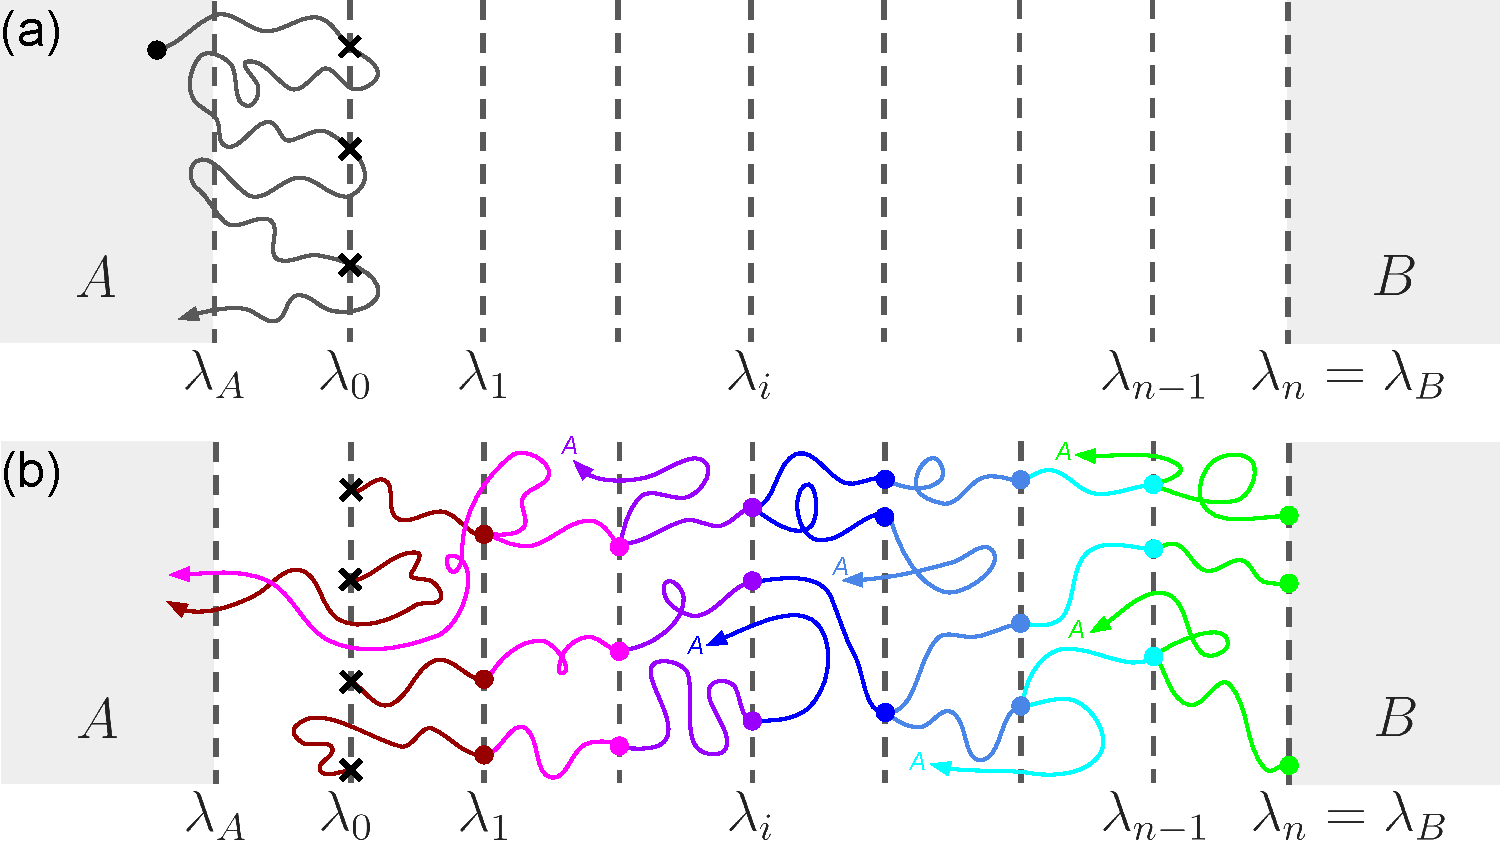
\includegraphics[width=\textwidth]{ffs_schematic.pdf}
\caption{Schematic of the Forward Flux Sampling algorithm (after \citealt{allen2006forward}).
\textit{Left panel (flux phase)}: Trajectories from state $A$ (gray, $Q > 1008$~hPa) evolve
forward in time; decorrelated crossings of $\lambda_0$ (orange circles) are saved.
Trajectories reaching state $B$ directly are tallied for direct-sampling rate validation.
\textit{Right panel (shooting phase)}: Trajectories launched from saved $\lambda_i$ configurations
either return to $A$ (purple; failed) or advance to $\lambda_{i+1}$ (dark blue; success), yielding
$P(\lambda_{i+1}|\lambda_i)$. The genesis rate is $k = \Phi_{A,0}\prod_i P(\lambda_{i+1}|\lambda_i)$.}
\label{fig:schematic}
\end{figure}

\section{Results}

\subsection{Seasonal Genesis Rates and Internal Validation}

Figure~\ref{fig:rates} shows FFS genesis rates across all 98 initial conditions.
The full seasonal cycle spans nearly three orders of magnitude,
from $2.6\times10^{-5}$~day$^{-1}$ during suppressed October conditions to
$1.7\times10^{-2}$~day$^{-1}$ during the peak-activity period around September~9--10
(consistent with the Fiona formation environment). This dynamic range is entirely unresolvable by direct 50-member ensemble sampling.
For context, the ECMWF IFS 50-member ensemble analyzed over the same 98 initial
conditions reaches the minimum MSLP threshold in 25.4\% of members on average;
this figure is included in Figure~\ref{fig:rates} as a \textit{qualitative sanity check}
only. A direct rate comparison between FFS (SDL-WXFormer, 1$^\circ$) and IFS
(0.25$^\circ$ physics, 1.5$^\circ$ output) is not appropriate: IFS does not apply
the decorrelated-crossing requirement defining $\lambda_0$ flux, does not use a CPS
filter, and operates at different resolution with different physics.
The IFS figures confirm that strong MSLP deepening occurs in the model at a
plausible frequency; quantitative rate comparisons between the two systems
are deferred to future work with matched configurations.

The primary internal validation is the agreement between $k^{\text{FFS}}$ and the
independent direct-sampling rate $k^{\text{direct}}$ (Figure~\ref{fig:rate_scatter}).
These estimates are derived from entirely separate components of the same simulation:
$k^{\text{FFS}}$ is a product of flux and shooting probabilities, while $k^{\text{direct}}$
counts raw state-$B$ arrivals during the flux phase.
Across all 98 initial conditions, the ratio $k^{\text{FFS}}/k^{\text{direct}} = 1.03 \pm 0.15$
(mean $\pm$ std; median 1.00; range 0.71--1.52; Figure~\ref{fig:rate_scatter}).
The near-unity mean and median indicate no systematic bias in the factorization.
The standard deviation of 0.15 and the factor-of-two range reflect the Poisson
sampling noise inherent in $k^{\text{direct}}$ (which has few counts at suppressed ICs),
not a bias in $k^{\text{FFS}}$.
Critically, this agreement holds across three orders of magnitude of genesis probability,
which would be expected only if (1) the interface spacing produces well-conditioned
probability estimates, (2) the ensemble sizes are adequate, and (3) the CPS screen
does not introduce systematic bias.
We interpret this agreement as self-consistency validation within the SDL-WXFormer
framework; it does not constitute verification against observed climatology.

\textbf{Markovianity.}
FFS requires Markovian dynamics: a trajectory's future behaviour must depend only
on its current state, not on its history prior to the most recent interface crossing.
We test this implicitly through the self-consistency validation: if significant
memory effects were present across interfaces, the FFS product $\Phi_{A,0}\prod P_i$
would systematically over- or under-estimate $k^{\text{direct}}$ (which contains no
interface-level conditioning). The near-unity ratio across 98 ICs constitutes an
empirical trajectory-level test — the most direct available within this framework.
We note that the observed anti-correlation between $P_1$ and $P_4$ across ICs
(environments favorable for initial organisation tend to have suppressed final-stage
probabilities) reflects \textit{cross-IC} atmospheric variability, not within-trajectory
memory, and does not violate Markovianity. A more rigorous test --- comparing
conditional probabilities for trajectories with different histories at the same interface
--- is deferred to future work but is not indicated by the current validation results.

Computational enhancement factors range from $3\times$ (most active IC) to $140\times$
(most suppressed), with geometric mean $14\times$.

\begin{figure}[htbp]
\centering
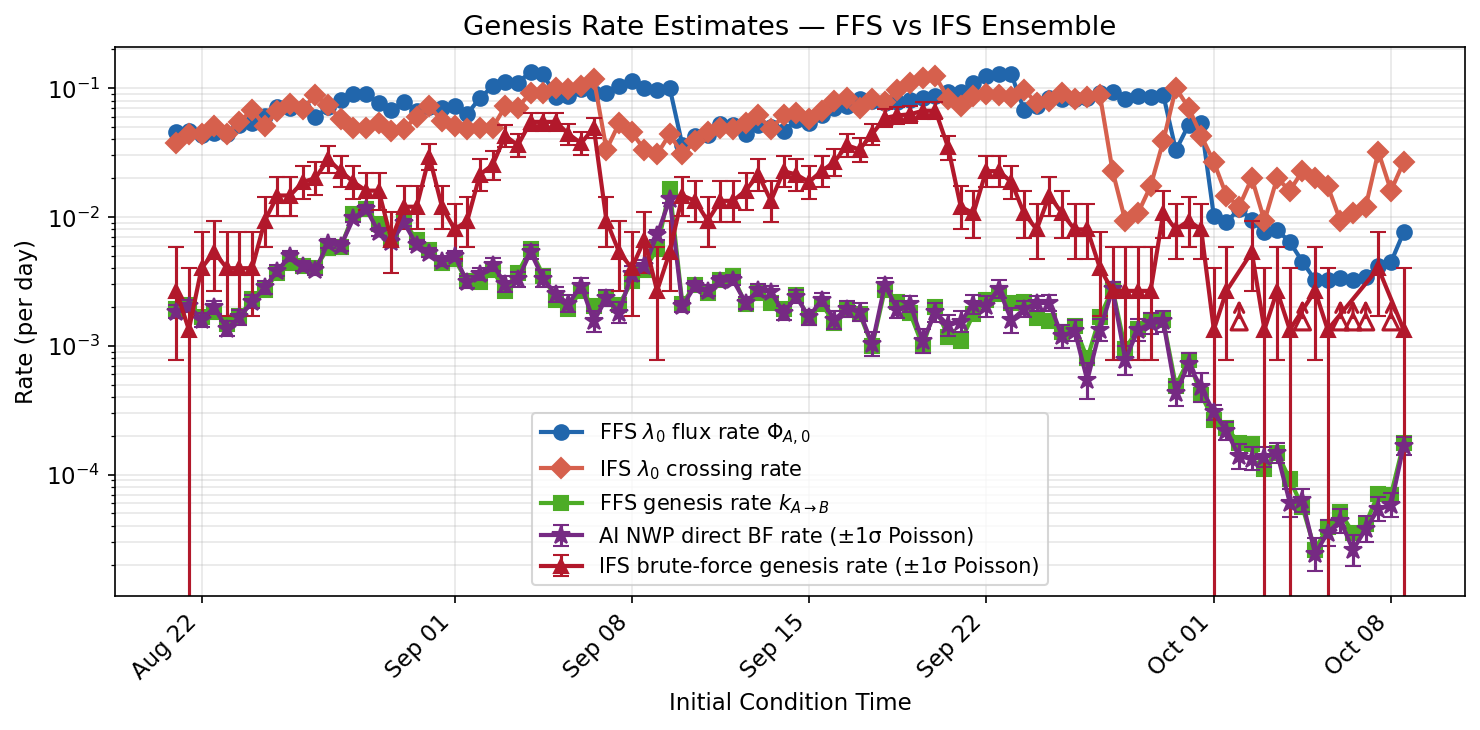
\includegraphics[width=\textwidth]{rates_plot.png}
\caption{FFS genesis rates across all 98 initial conditions (August~21 -- October~8, 2022)
on a logarithmic scale.
\textit{Blue}: $\lambda_0$ flux rate $\Phi_{A,0}$.
\textit{Orange}: IFS $\lambda_0$ crossing rate (contextual reference; not directly comparable to FFS due to different resolution and no CPS filter).
\textit{Green}: Full FFS genesis rate $k^{\text{FFS}}$ (flux $\times$ product of conditional probabilities).
\textit{Purple}: Direct-sampling rate $k^{\text{direct}}$ from state-$B$ arrivals during the flux phase ($\pm 1\sigma$ Poisson).
\textit{Red}: IFS brute-force genesis rate ($\pm 1\sigma$ Poisson; upward arrows denote upper bounds where zero events observed).
Agreement between green and purple (mean ratio $1.03\pm0.15$) validates the FFS method.
The FFS rate resolves a seasonal cycle spanning nearly three orders of magnitude
invisible to direct 50-member ensemble sampling.}
\label{fig:rates}
\end{figure}

\begin{figure}[htbp]
\centering
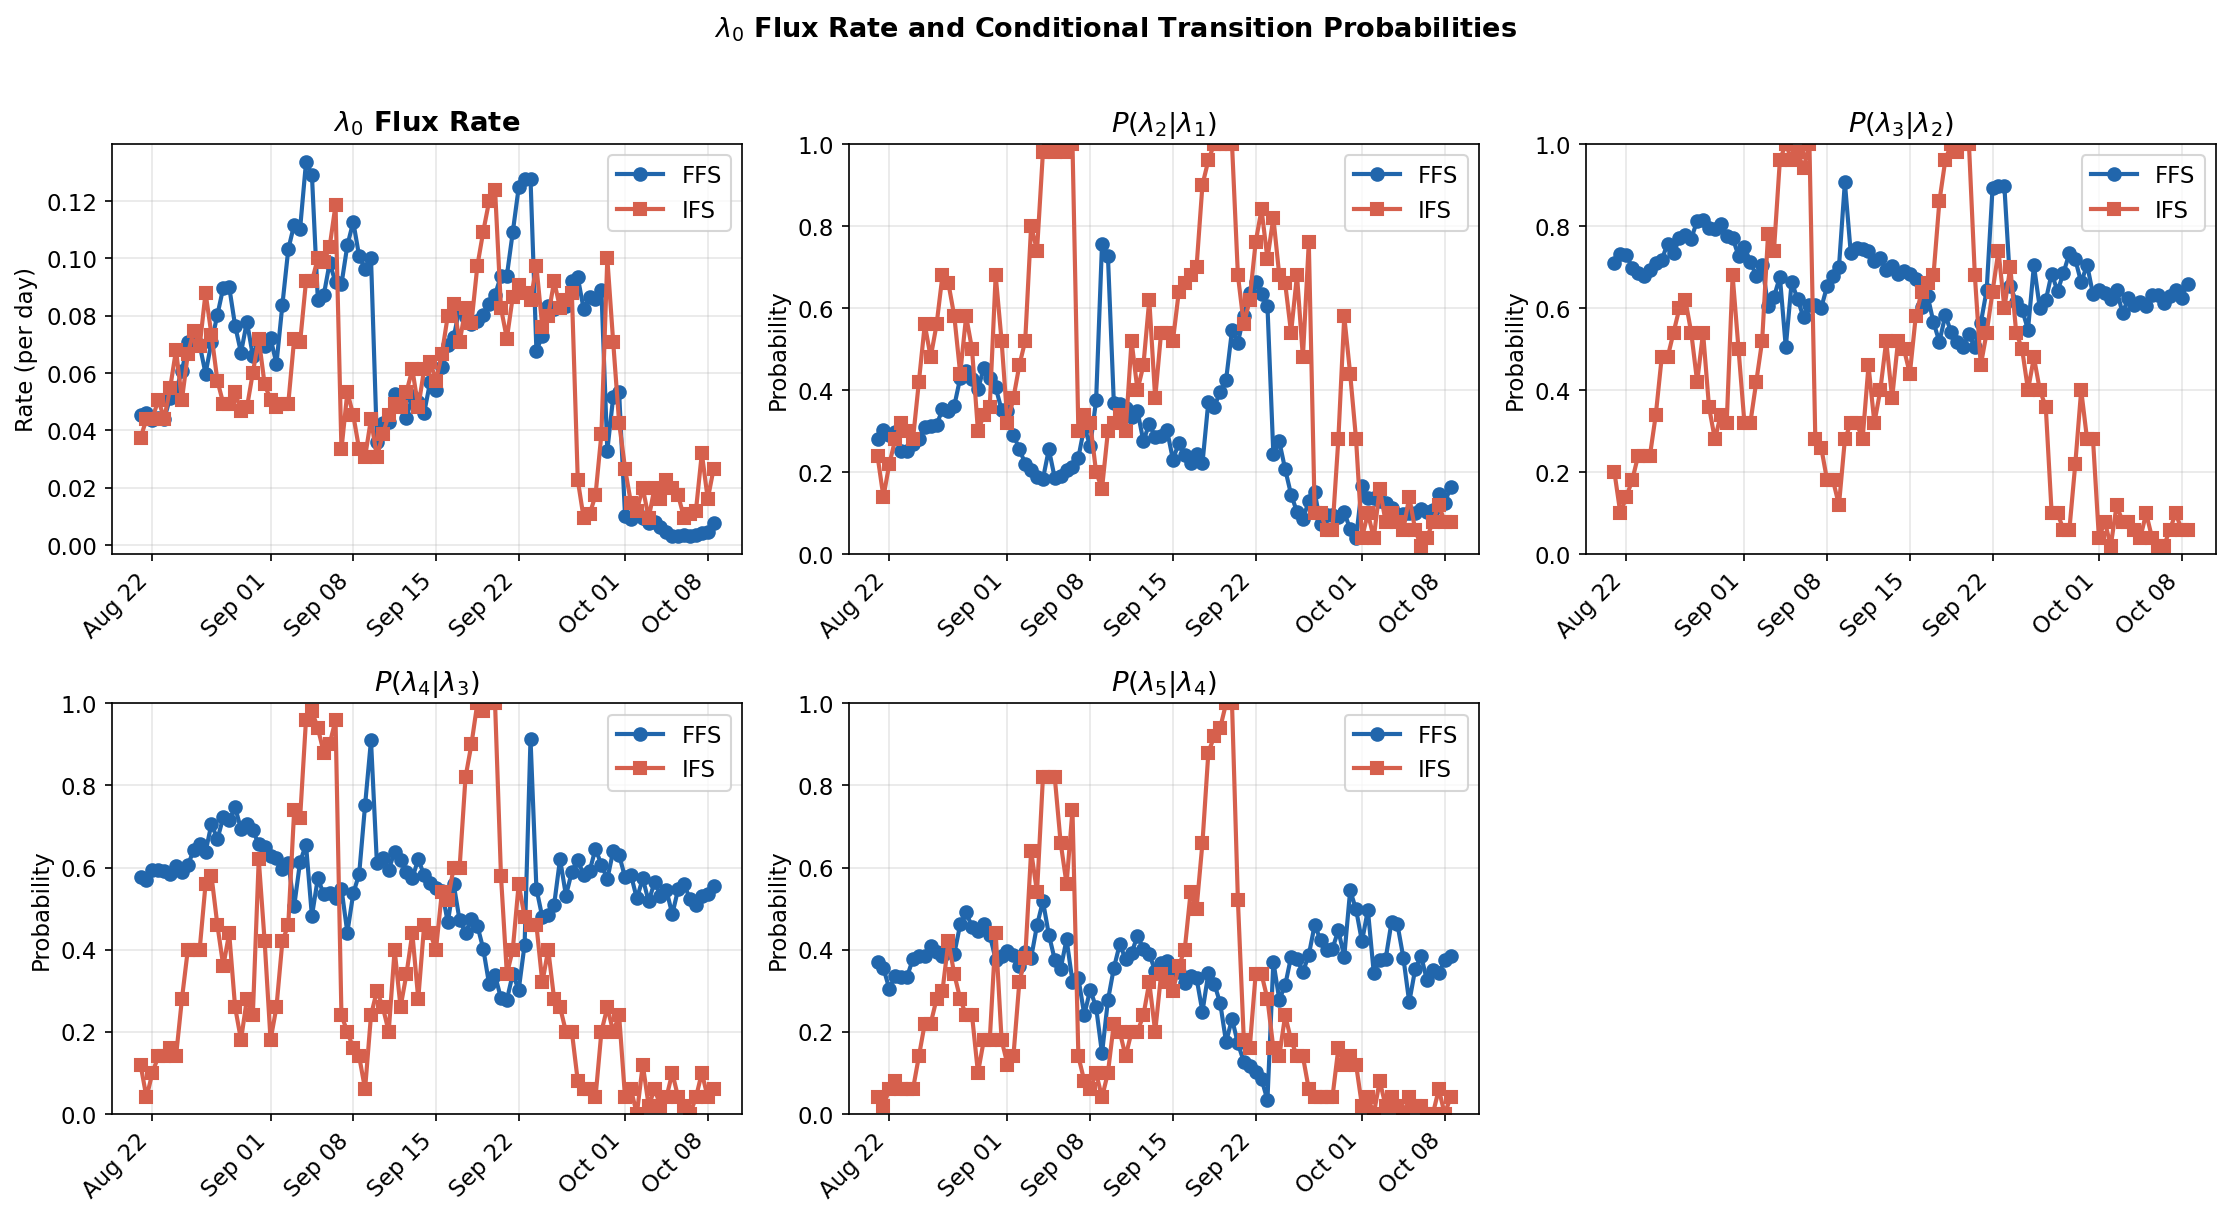
\includegraphics[width=\textwidth]{ffs_interface_probs.png}
\caption{Seasonal evolution of FFS conditional crossing probabilities $P(\lambda_i|\lambda_{i-1})$
for all 98 initial conditions (August~21 -- October~8, 2022). The first panel shows the $\lambda_0$
flux rate; subsequent panels show each $P_i$ between successive shooting interfaces.
The dashed line marks the all-season mean. $P_1$ (initial organization, $\lambda_1\to\lambda_2$)
varies most strongly with the seasonal cycle, with a pronounced peak in early September coinciding
with the Fiona formation environment. $P_4$ (final intensification, $\lambda_4\to B$) is
the most uniformly suppressed probability, limiting the overall genesis rate even in active periods.
The three case-study ICs (Earl~09-02, active~09-09, Ian~09-22) are indicated by vertical markers.}
\label{fig:interface_probs}
\end{figure}

\begin{figure}[htbp]
\centering
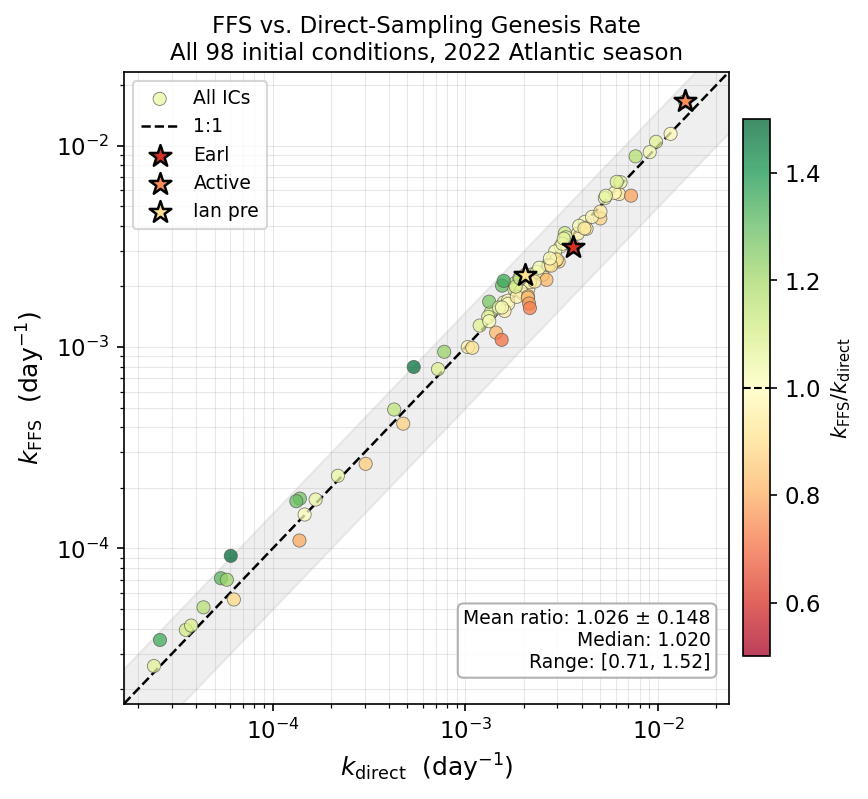
\includegraphics[width=\textwidth]{ffs_vs_direct_scatter.png}
\caption{Log-log scatter of FFS genesis rate $k^{\text{FFS}}$ versus independent
direct-sampling rate $k^{\text{direct}}$ for all 98 initial conditions.
Points are coloured by the ratio $k^{\text{FFS}}/k^{\text{direct}}$: green indicates
near-unity agreement; red/blue indicate over- or under-estimation.
The black dashed line is the 1:1 reference; shaded band spans $\pm$50\%.
Three case-study ICs are marked with stars (Earl: red; active: orange; Ian~pre: yellow).
The tight clustering along the 1:1 line across three orders of magnitude confirms
correct implementation of the conditional probability factorization.
Inset statistics: mean ratio $1.03\pm0.15$, median $1.00$, range $[0.71, 1.52]$.}
\label{fig:rate_scatter}
\end{figure}

\begin{figure}[htbp]
\centering
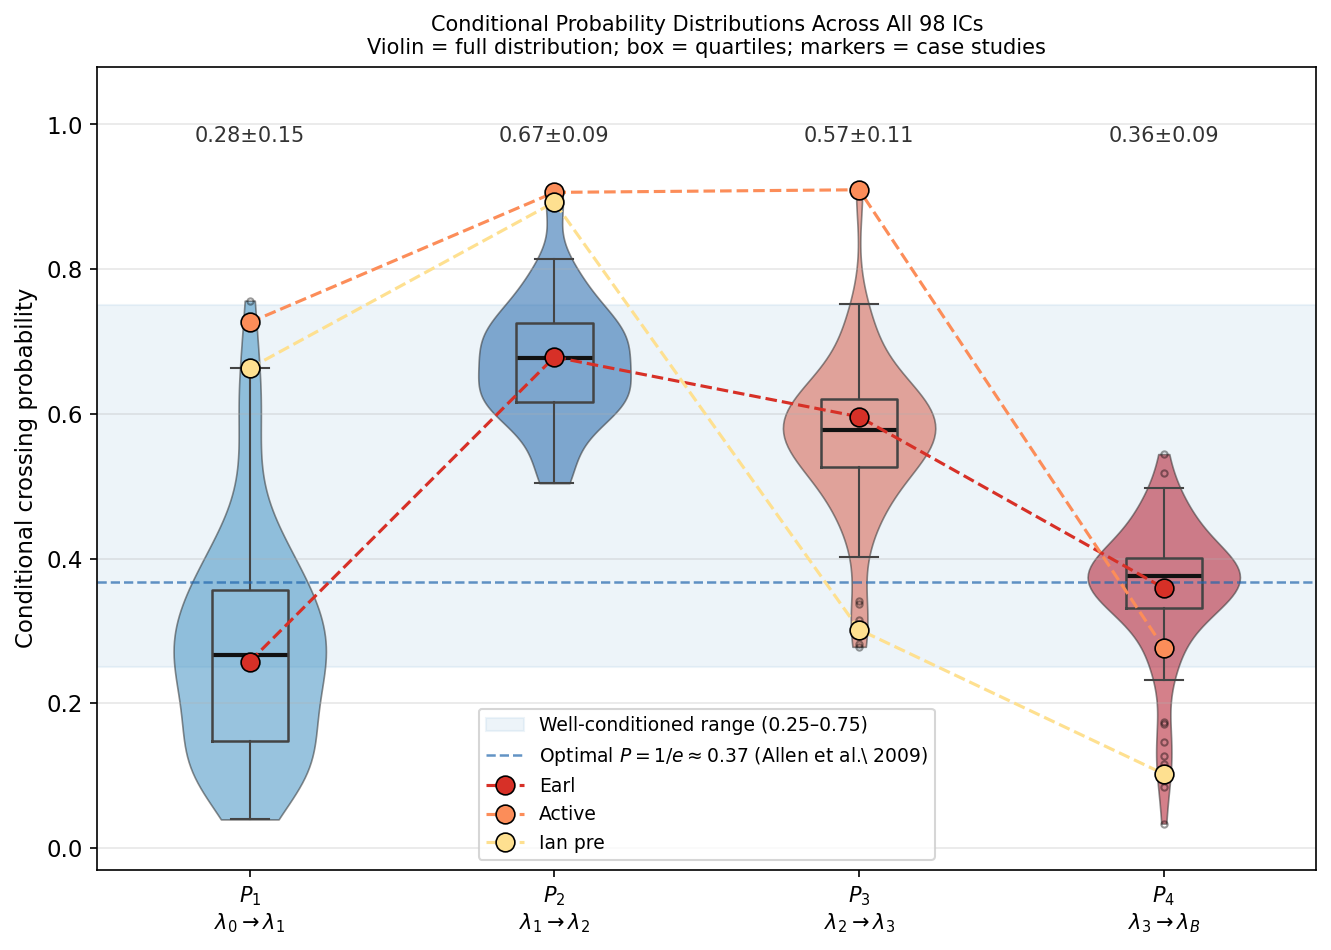
\includegraphics[width=\textwidth]{conditional_prob_distributions.png}
\caption{Distribution of conditional crossing probabilities $P_i$ across all 98 initial
conditions. Each violin shows the full distribution; boxes show quartiles; coloured
lines connect the three case-study ICs. The horizontal dashed line marks the optimal
$P = 1/e \approx 0.37$ (Kratzer et al.); the blue band spans the target range 0.25--0.55.
Most ICs have $P_i$ within the well-conditioned range, confirming that interface placement
produces efficient variance reduction. The spread of $P_1$ (initial organization) is larger
than that of $P_2$--$P_3$, reflecting the dominant role of large-scale atmospheric variability
in setting the first intensification barrier. Mean $\pm$ SD for each interface are annotated.}
\label{fig:cond_prob_dist}
\end{figure}

\subsection{Case Studies: Distinct Genesis Bottlenecks}

Table~\ref{tab:results} presents FFS statistics for the three case-study initial
conditions. The most striking feature is the variable position of the rate-limiting
step, encoded in which conditional probability is smallest.
Figure~\ref{fig:stateb_geo} shows the geographic distribution of state-$B$ arrivals
across all 98 ICs, confirming that the model's genesis events cluster in physically
plausible locations (tropical Atlantic, Caribbean, Gulf of Mexico) and shift
geographically with the seasonal cycle.

\begin{table}[htbp]
\centering
\caption{FFS statistics for three case-study initial conditions.
$\Phi_{A,0}$: flux rate. $P_i$: conditional crossing probability at interface $\lambda_i$.
$k^{\text{FFS}}$: full genesis rate (Eq.~\ref{eq:ffs_rate}). $k^{\text{direct}}$:
independent direct-sampling rate. Ratio: $k^{\text{FFS}}/k^{\text{direct}}$.
Speedup: enhancement over direct sampling for equivalent 20\% rate uncertainty.
Bottom row: statistics across all 98 ICs.}
\label{tab:results}
\resizebox{\textwidth}{!}{%
\begin{tabular}{lccccccccc}
\toprule
IC & $\Phi_{A,0}$ & $P_1$ & $P_2$ & $P_3$ & $P_4$ & $k^{\text{FFS}}$ & $k^{\text{direct}}$ & Ratio & Speedup \\
   & (day$^{-1}$) & & & & & (day$^{-1}$) & (day$^{-1}$) & & \\
\midrule
Earl (09-02T00Z)    & 0.0837 & \textbf{0.258} & 0.679 & 0.596 & 0.359 & $3.13\times10^{-3}$ & $3.61\times10^{-3}$ & 0.87 & 10$\times$ \\
Active (09-09T12Z)  & 0.1002 & 0.726 & 0.906 & 0.910 & \textbf{0.276} & $1.66\times10^{-2}$ & $1.37\times10^{-2}$ & 1.21 &  3$\times$ \\
Ian pre. (09-22T00Z) & 0.1247 & 0.663 & 0.893 & \textbf{0.302} & \textbf{0.102} & $2.28\times10^{-3}$ & $2.04\times10^{-3}$ & 1.12 & 19$\times$ \\
\midrule
All-98 mean$\pm$SD  & $0.065\pm0.034$ & $0.278\pm0.154$ & $0.674\pm0.086$ & $0.569\pm0.107$ & $0.356\pm0.093$ & $2.6\times10^{-3}$ & $2.5\times10^{-3}$ & $1.03\pm0.15$ & $14\times$$^{\dagger}$ \\
\bottomrule
\multicolumn{10}{l}{$^{\dagger}$Geometric mean; range 3--140$\times$. Speedup distribution is right-skewed; geometric mean is the appropriate summary.}
\end{tabular}%
}
\end{table}

For the \textbf{Earl IC}, $P_1 = 0.258$ is the dominant bottleneck: fewer than 1 in 4
trajectories crossing 1000~hPa organize to 987~hPa in this environment. This is
physically consistent with the pre-genesis atmospheric state $\sim$24~hours before
Earl's classification, when the system had established a coherent low-level circulation
but had not yet achieved the sustained convective organization needed to cross the
first intensification threshold.

For the \textbf{active-period IC} (September~9), all four conditional probabilities
are elevated ($\geq0.28$), and the product $\prod P_i = 0.166$ is $\sim$4--9$\times$
larger than the other two cases. The dominant bottleneck shifts to $P_4 = 0.276$
(final intensification to 975~hPa), reflecting an environment that readily organizes
disturbances but where crossing the hurricane-threshold step remains non-trivial.
The FFS rate ($1.66\times10^{-2}$~day$^{-1}$) is high enough that direct sampling
is also feasible (speedup $3\times$), providing a strong cross-validation: both methods
agree to within 21\% for this most-active IC.

The \textbf{Ian precursor IC} presents the most physically interesting pattern.
$P_1 = 0.663$ and $P_2 = 0.893$ indicate that the environment readily supports initial
organization through 985~hPa, consistent with the warm, moist, low-shear conditions
present over the Caribbean and western Atlantic on September~22. But $P_3 = 0.302$
and $P_4 = 0.102$ reveal a hard barrier in the final intensification steps (981~hPa
to 975~hPa). This is physically consistent with Ian's trajectory: the storm was still
organizing over the Caribbean on September~22--23, entering the Gulf of Mexico's warm
core environment only after September~25, when conditions supported rapid intensification.
The FFS framework identifies the final-stage intensification barrier \textit{one day before}
Ian's official genesis --- a diagnostic that direct ensemble sampling cannot resolve.

\begin{figure}[htbp]
\centering
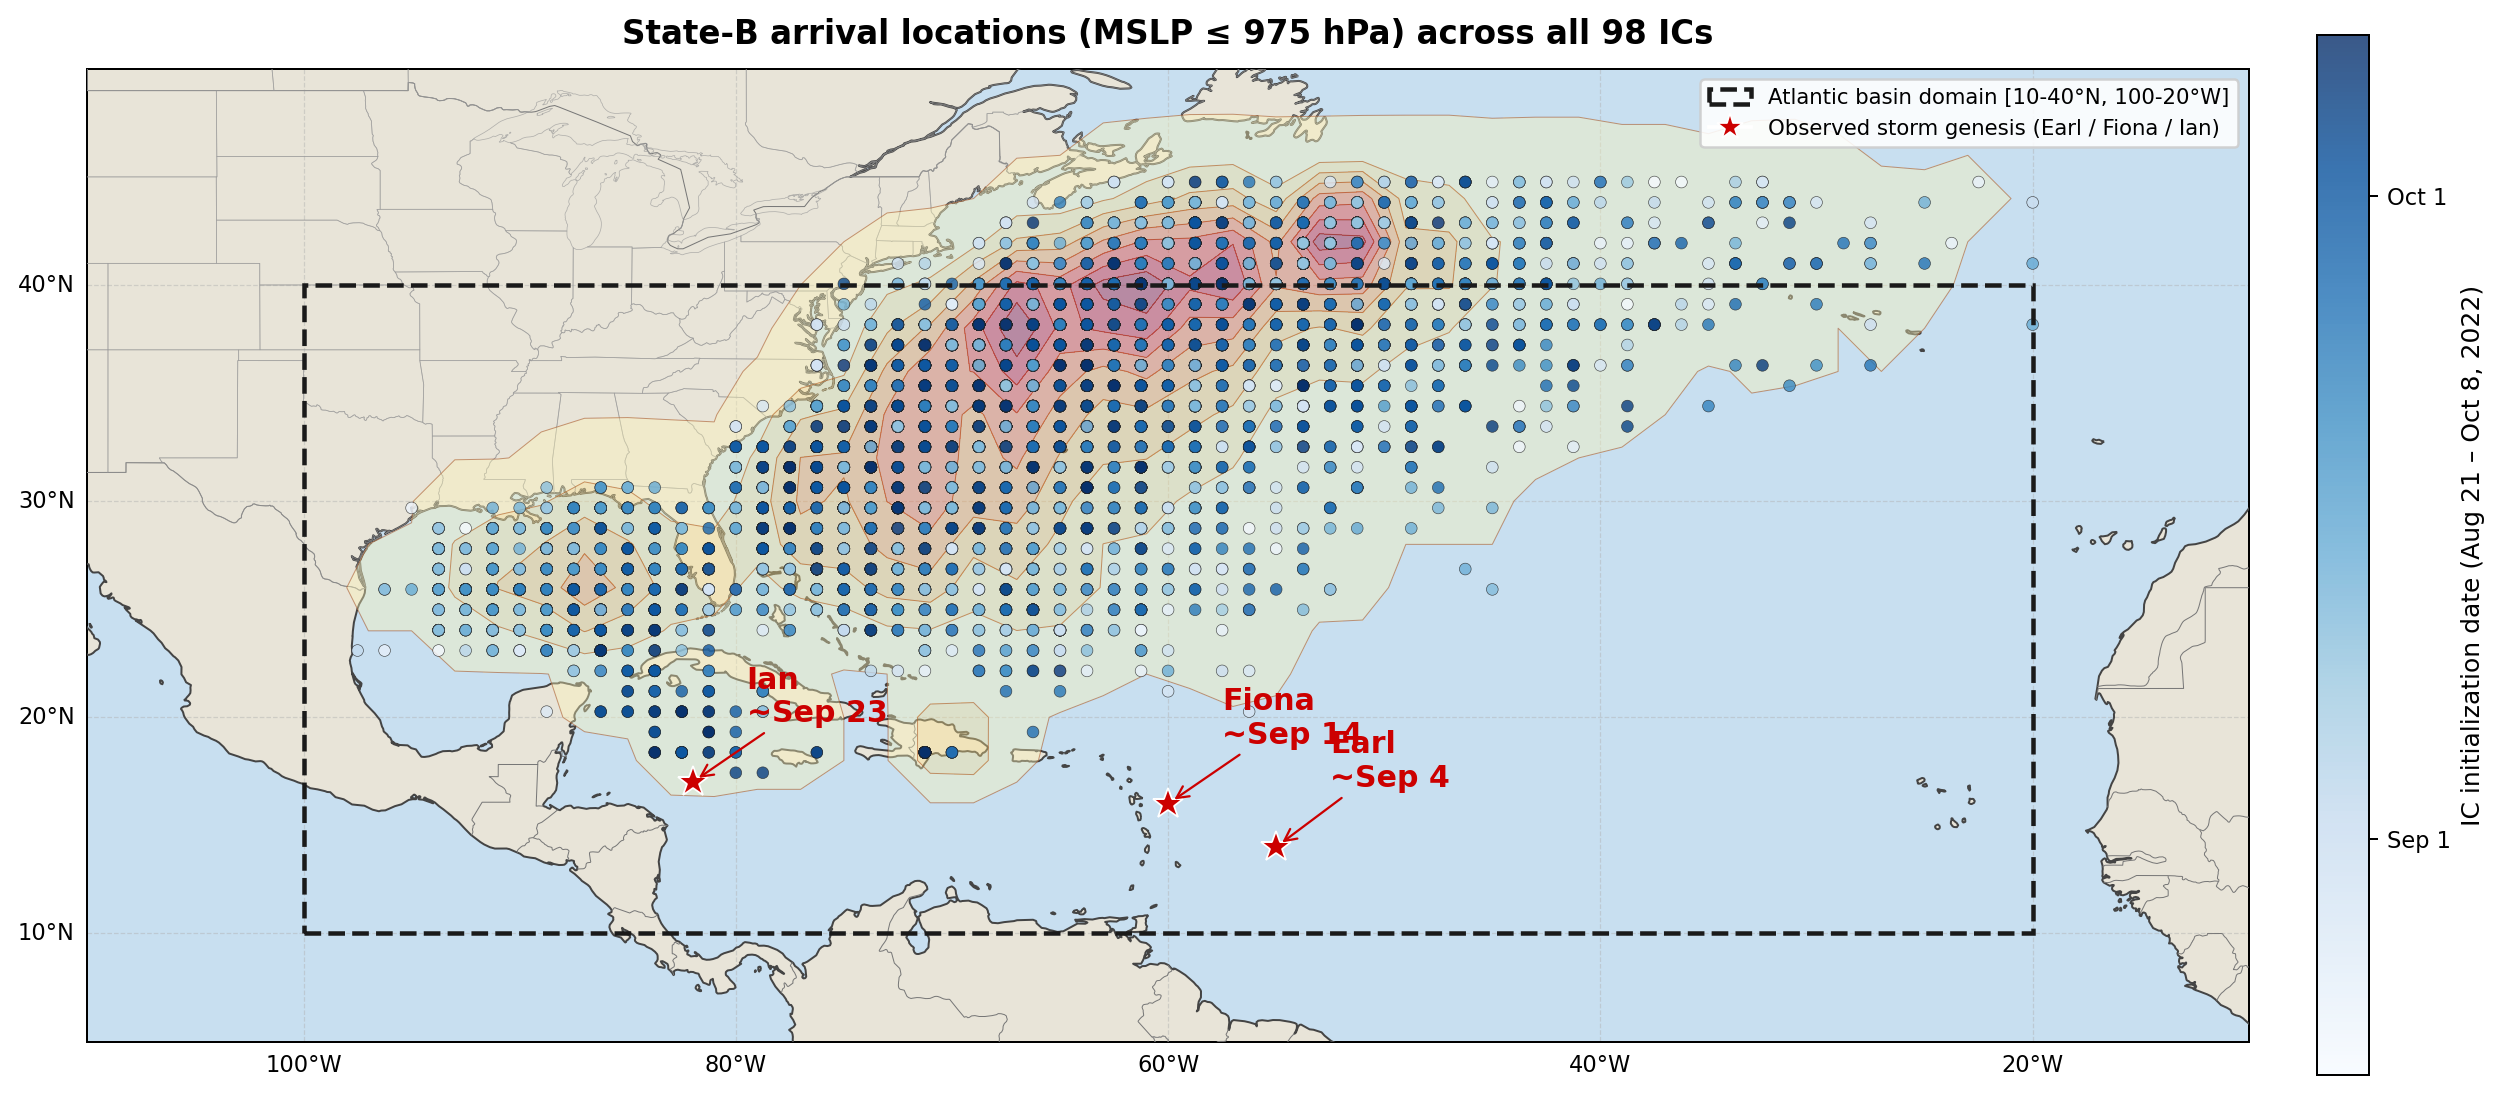
\includegraphics[width=\textwidth]{stateb_geography.png}
\caption{Geographic distribution of state-$B$ arrival locations (MSLP $\leq$ 975~hPa)
across all 98 initial conditions.
Each point marks where a reactive trajectory first reached state~$B$; colour encodes
the IC initialisation date from August~21 (light) to October~8 (dark).
The 2$^\circ$ density contours (background) show the spatial clustering of genesis events
across the season. Approximate observed genesis locations for Earl, Fiona, and Ian are
annotated for reference. The distribution is concentrated in the tropical Atlantic,
Caribbean, and Gulf of Mexico, consistent with observed 2022 Atlantic storm tracks,
and shifts westward later in the season as Ian-like Gulf environments become active.}
\label{fig:stateb_geo}
\end{figure}

\begin{figure}[htbp]
\centering
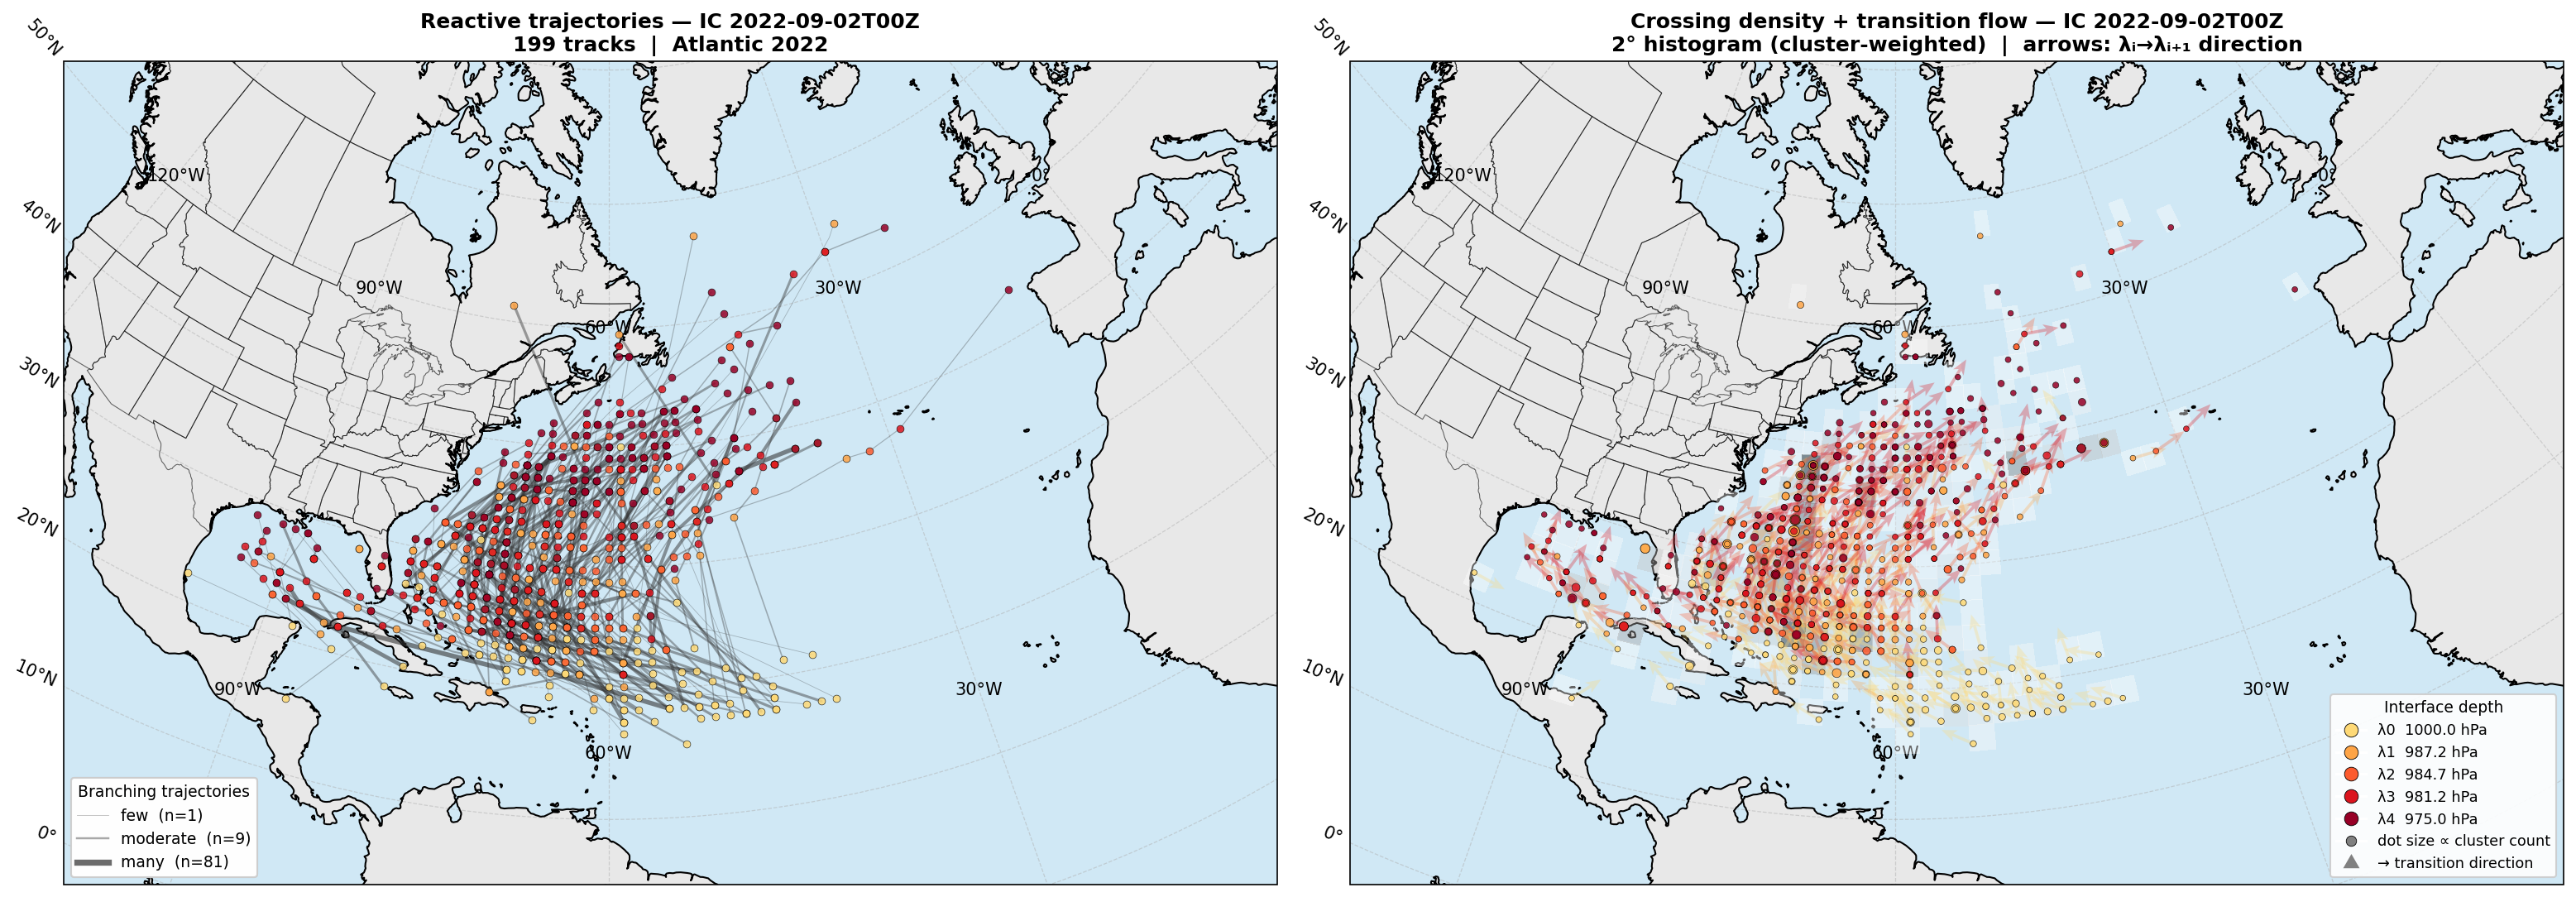
\includegraphics[width=\textwidth]{reactive_trajectories_2022-09-02T00Z.png}
\caption{Reactive genesis trajectories for the Earl IC (2022-09-02T00Z).
\textit{Left}: Individual tracks that cross from $\lambda_0$ through to state~$B$,
color-coded by branching factor (cluster weight); the 199 reactive pathways sample
a broad region spanning the tropical Atlantic, Caribbean, and western subtropical Atlantic.
\textit{Right}: Cluster-weighted crossing density (2$^\circ$ histogram) and mean
$\lambda_n\to\lambda_{n+1}$ transition direction (arrows), revealing the geographic regions
most active in the intensification cascade for this environment.
CPS-rejected (extratropical) trajectories are excluded from both panels.}
\label{fig:reactive_traj}
\end{figure}

\subsection{FFS Shooting Trees}

Figure~\ref{fig:ffs_trees} shows representative FFS shooting trees for each of the three
case-study ICs. Each tree traces the branching genealogy of a single $\lambda_0$ seed:
the star marks the seed location, and successive interface crossings fan out as the
ensemble of reactive pathways progresses toward state~$B$.
The geographic spread of $\lambda_4$ descendants reflects the diversity of intensification
pathways sampled by the FFS from a single starting configuration.

Importantly, the IC date labels (09-02, 09-09, 09-22) are \textit{initialisation} times,
not genesis dates. Each FFS simulation runs 15 days forward from its IC; each node in the
tree represents the storm feature at a different future lead time within that window.
A single seed at $\lambda_0$ therefore spawns descendants that span a range of calendar
dates, geographic positions, and atmospheric states — all sampled from one background IC.

The Earl tree (left) originates near 31$^\circ$N in the western Atlantic and fans
northeastward, sampling the open Atlantic development region.
The Fiona precursor tree (centre) seeds near 19$^\circ$N in the open Atlantic and
fans northwestward toward the Caribbean and Bahamas; Fiona was designated a tropical
storm on September~14 --- five days into this simulation window.
The Ian precursor tree (right) seeds near 18$^\circ$N in the Caribbean and fans
northwestward into the Gulf of Mexico, directly anticipating Ian's observed path.

\begin{figure}[htbp]
\centering
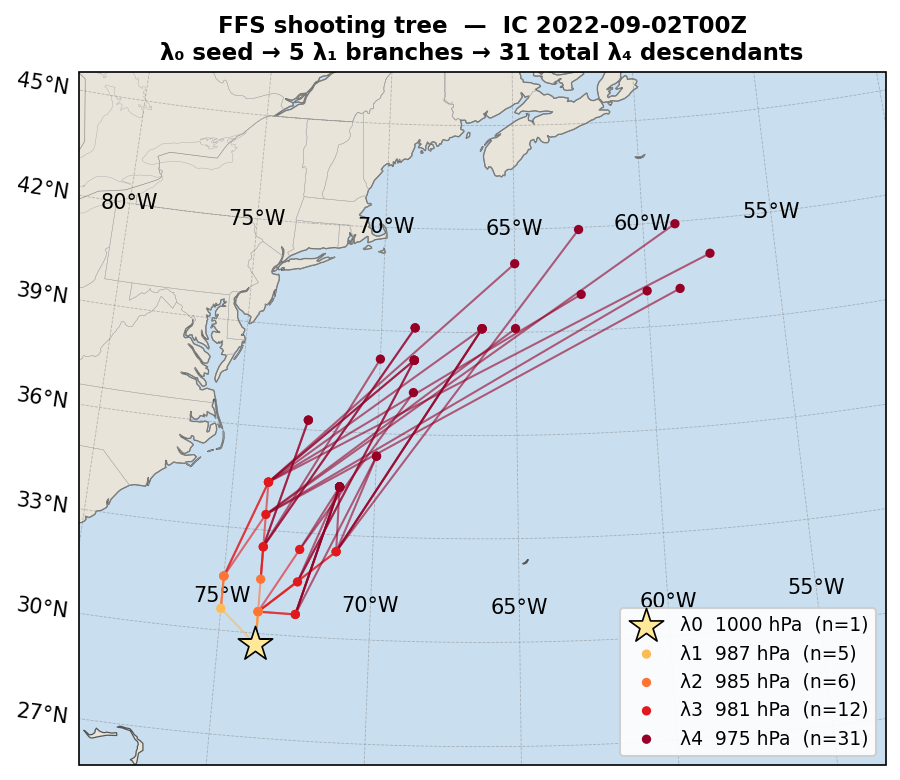
\includegraphics[height=5cm]{ffs_tree_rank05_2022-09-02T00Z_lambda0_config_0175_JR.png}\hfill
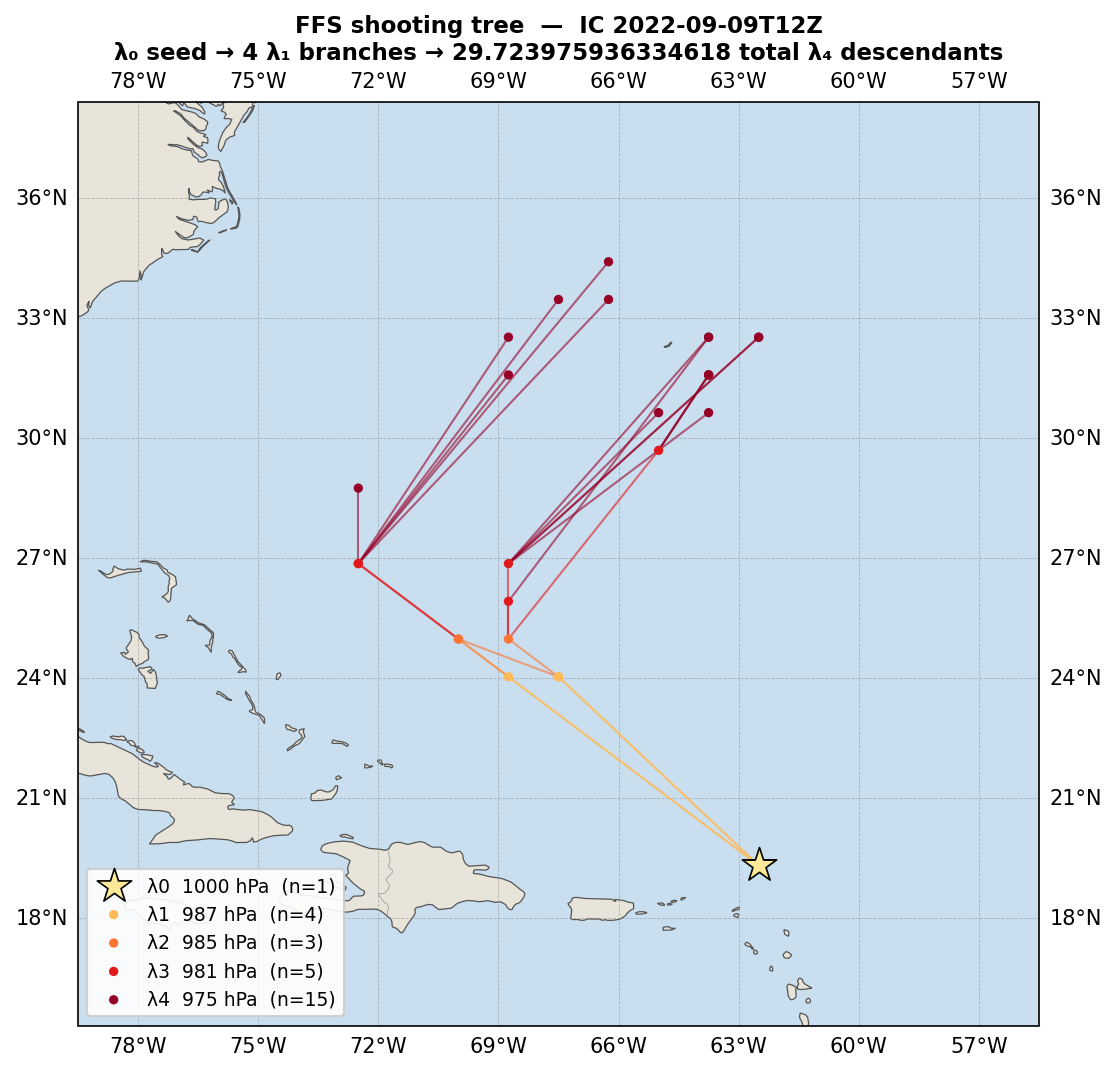
\includegraphics[height=5cm]{ffs_tree_rank04_2022-09-09T12Z_lambda0_config_0545_MZ.png}\hfill
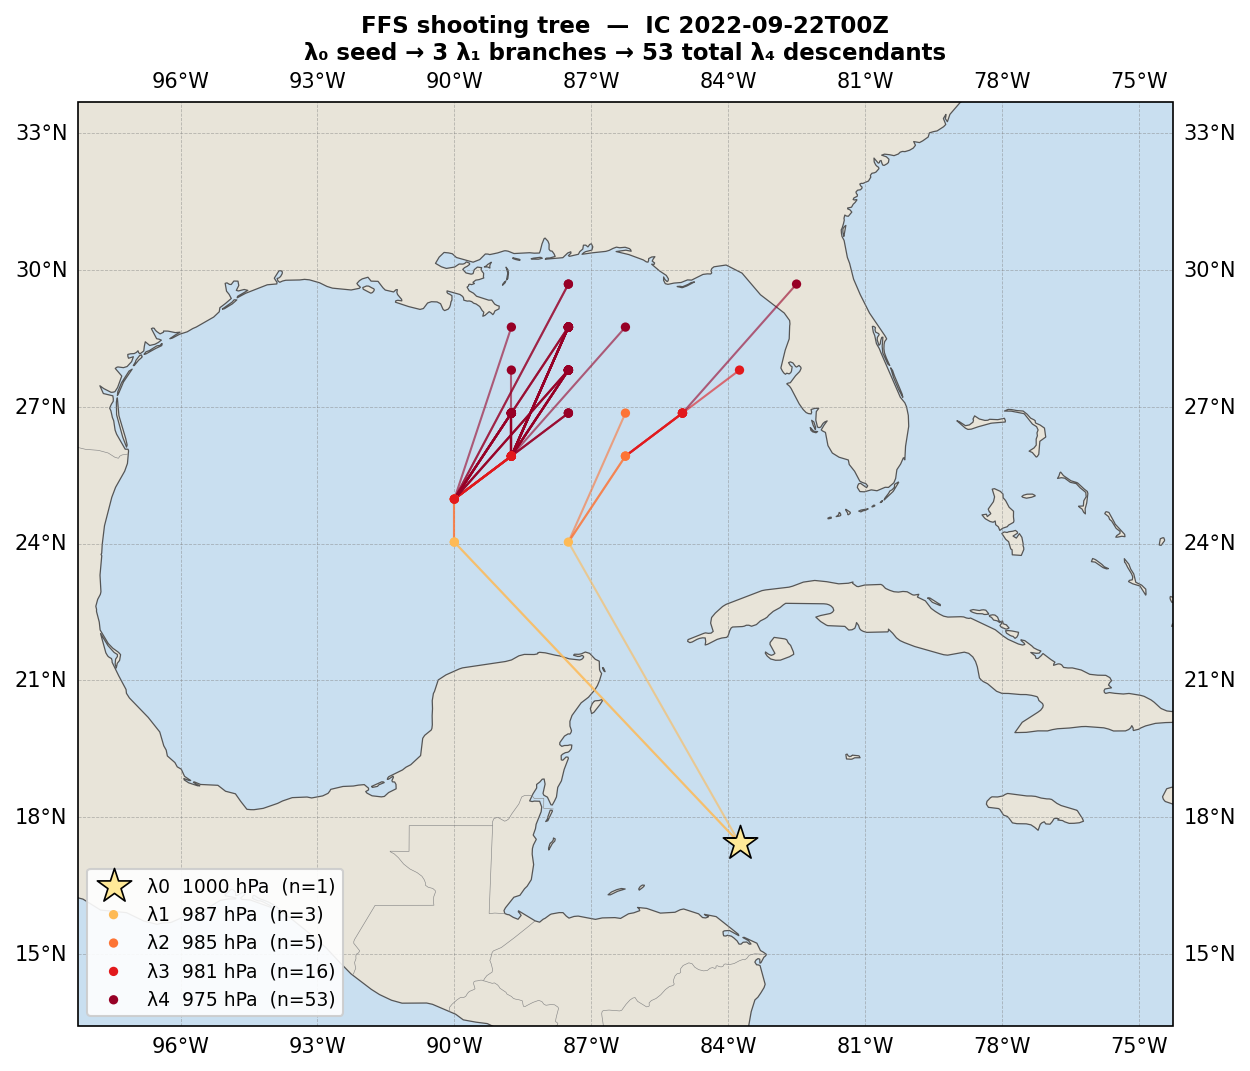
\includegraphics[height=5cm]{ffs_tree_rank02_2022-09-22T00Z_lambda0_config_0917_OV.png}
\caption{FFS shooting trees for the three case-study ICs (initialisation dates shown;
each simulation runs 15 days forward, so each node represents a different future
lead time within that window, not the IC date itself).
Each panel shows one $\lambda_0$ seed (star) and the branching cascade of interface
crossings to $\lambda_4$; marker colours indicate interface level.
\textit{Left}: Earl IC (init.\ 2022-09-02T00Z) — seed near 31$^\circ$N, 72$^\circ$W;
trajectories fan northeastward into the open Atlantic.
\textit{Centre}: Fiona precursor IC (init.\ 2022-09-09T12Z) — seed near 19$^\circ$N,
63$^\circ$W; Fiona was designated on day~5 of this window; trajectories track
northwestward consistent with its subsequent path.
\textit{Right}: Ian precursor IC (init.\ 2022-09-22T00Z) — seed near 18$^\circ$N,
84$^\circ$W; trajectories fan northwestward into the Gulf of Mexico, anticipating
Ian's observed track.}
\label{fig:ffs_trees}
\end{figure}

\subsection{Committor Curves and Spatial Genesis Fields}

Figure~\ref{fig:committor} shows the committor curve $p_B(\lambda_i)$ --- the probability
of eventually reaching state~$B$ given arrival at interface $\lambda_i$ --- averaged across
all 98 initial conditions for both the FFS (AI model) and IFS (brute-force ensemble).
The all-season FFS curve shows a near-linear decline with the steepest drop between
the first and second shooting interfaces ($\lambda_1\to\lambda_2$), consistent with the
seasonal mean of $P_1$ being the lowest of the four conditional probabilities
(Table~\ref{tab:results}).
The FFS and IFS curves agree in overall \textit{shape}: both show the steepest committor
drop at the same interface level, and both identify the same rate-limiting stage of the
intensification cascade.
This structural agreement --- across two completely independent modelling systems ---
provides suggestive cross-model consistency that the intensification bottleneck identified
by FFS reflects real atmospheric physics rather than artefacts of the SDL-WXFormer architecture;
we note that the comparison is complicated by the different ensemble generation mechanisms
(learned stochastic layers vs.\ singular-vector perturbations) and the 1$^\circ$ vs.\ 1.5$^\circ$
resolution asymmetry, so quantitative agreement is not expected and not claimed.
The FFS committors are systematically higher in \textit{magnitude}, consistent with
SDL-WXFormer's higher absolute genesis rate at 1$^\circ$ relative to IFS archived at 1.5$^\circ$
(the coarser IFS output smooths MSLP minima, effectively raising the intensification barrier).

\begin{figure}[htbp]
\centering
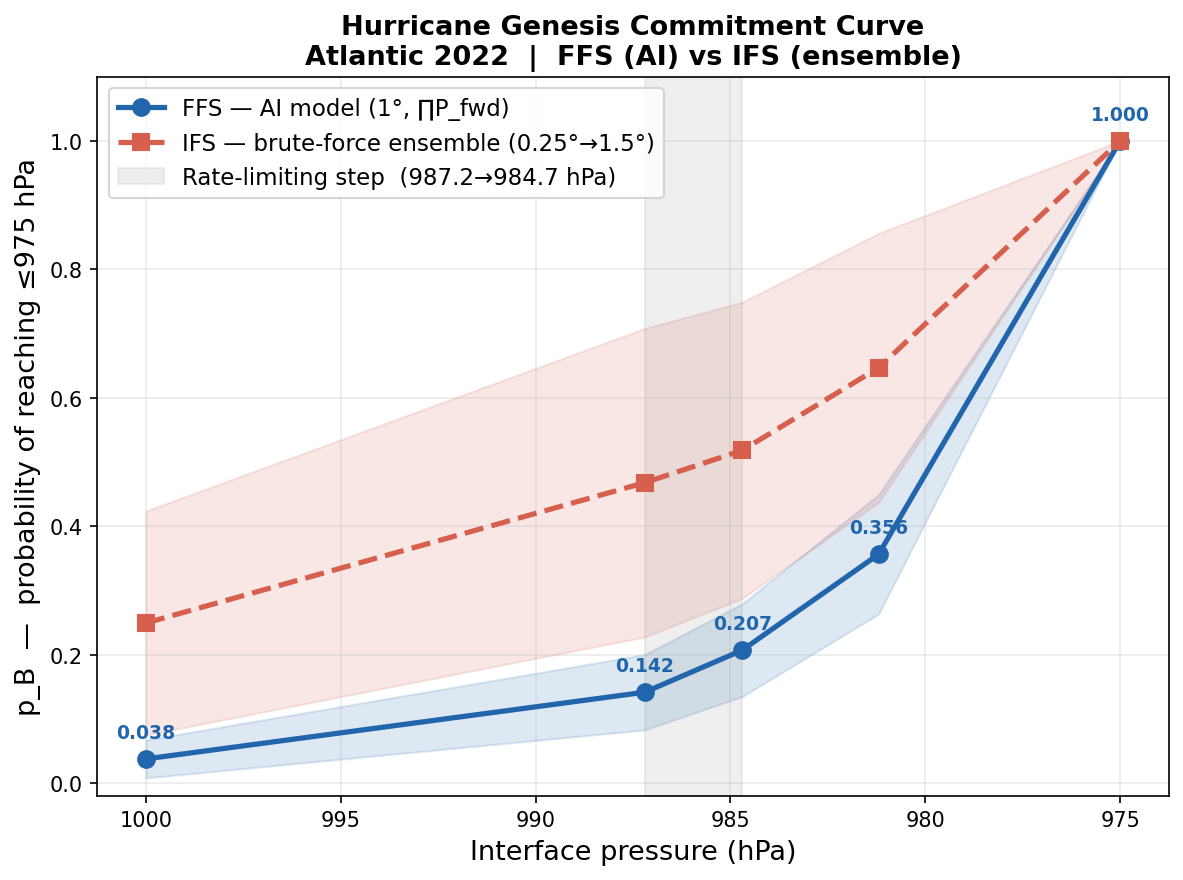
\includegraphics[width=0.85\textwidth]{commitment_curve.png}
\caption{Genesis committor curve $p_B(\lambda_i)$ — the probability of eventually reaching
state~$B$ ($\leq$975~hPa) given arrival at interface $\lambda_i$ — averaged across all 98
initial conditions.
\textit{Blue}: FFS AI model mean $\pm 1\sigma$ across ICs.
\textit{Orange}: IFS brute-force ensemble mean $\pm 1\sigma$ across ICs.
The shaded bands show IC-to-IC variability; the annotated values are the all-season FFS means.
The grey band highlights the rate-limiting step (largest single drop), which falls between
the first and second shooting interfaces for the full 2022 Atlantic season.
The FFS and IFS curves agree in the overall shape while differing in magnitude,
consistent with the resolution and physics differences between the two systems.}
\label{fig:committor}
\end{figure}

\subsection{Physics Along a Reactive Pathway}

Figure~\ref{fig:physics} traces the storm-centred thermodynamic and kinematic evolution
along a representative Earl reactive pathway (pathway~26) from $\lambda_0$ through state~$B$.
The vortex originates near 25$^\circ$N and tracks northeastward to 39$^\circ$N as it
intensifies from 998~hPa to 967~hPa, consistent with typical late-summer Atlantic
storm tracks in this environment.
The persistent cyclonic vorticity ($\zeta_{850}$) and warm-core anomaly ($T'_{500}$) at
each interface confirm continuous vortex identity and warm-core structure through state~$B$.
These storm-centred panels reveal the physical mechanisms operating at each stage,
connecting the abstract conditional probabilities in Table~\ref{tab:results} to concrete
dynamical processes.

\begin{figure}[htbp]
\centering
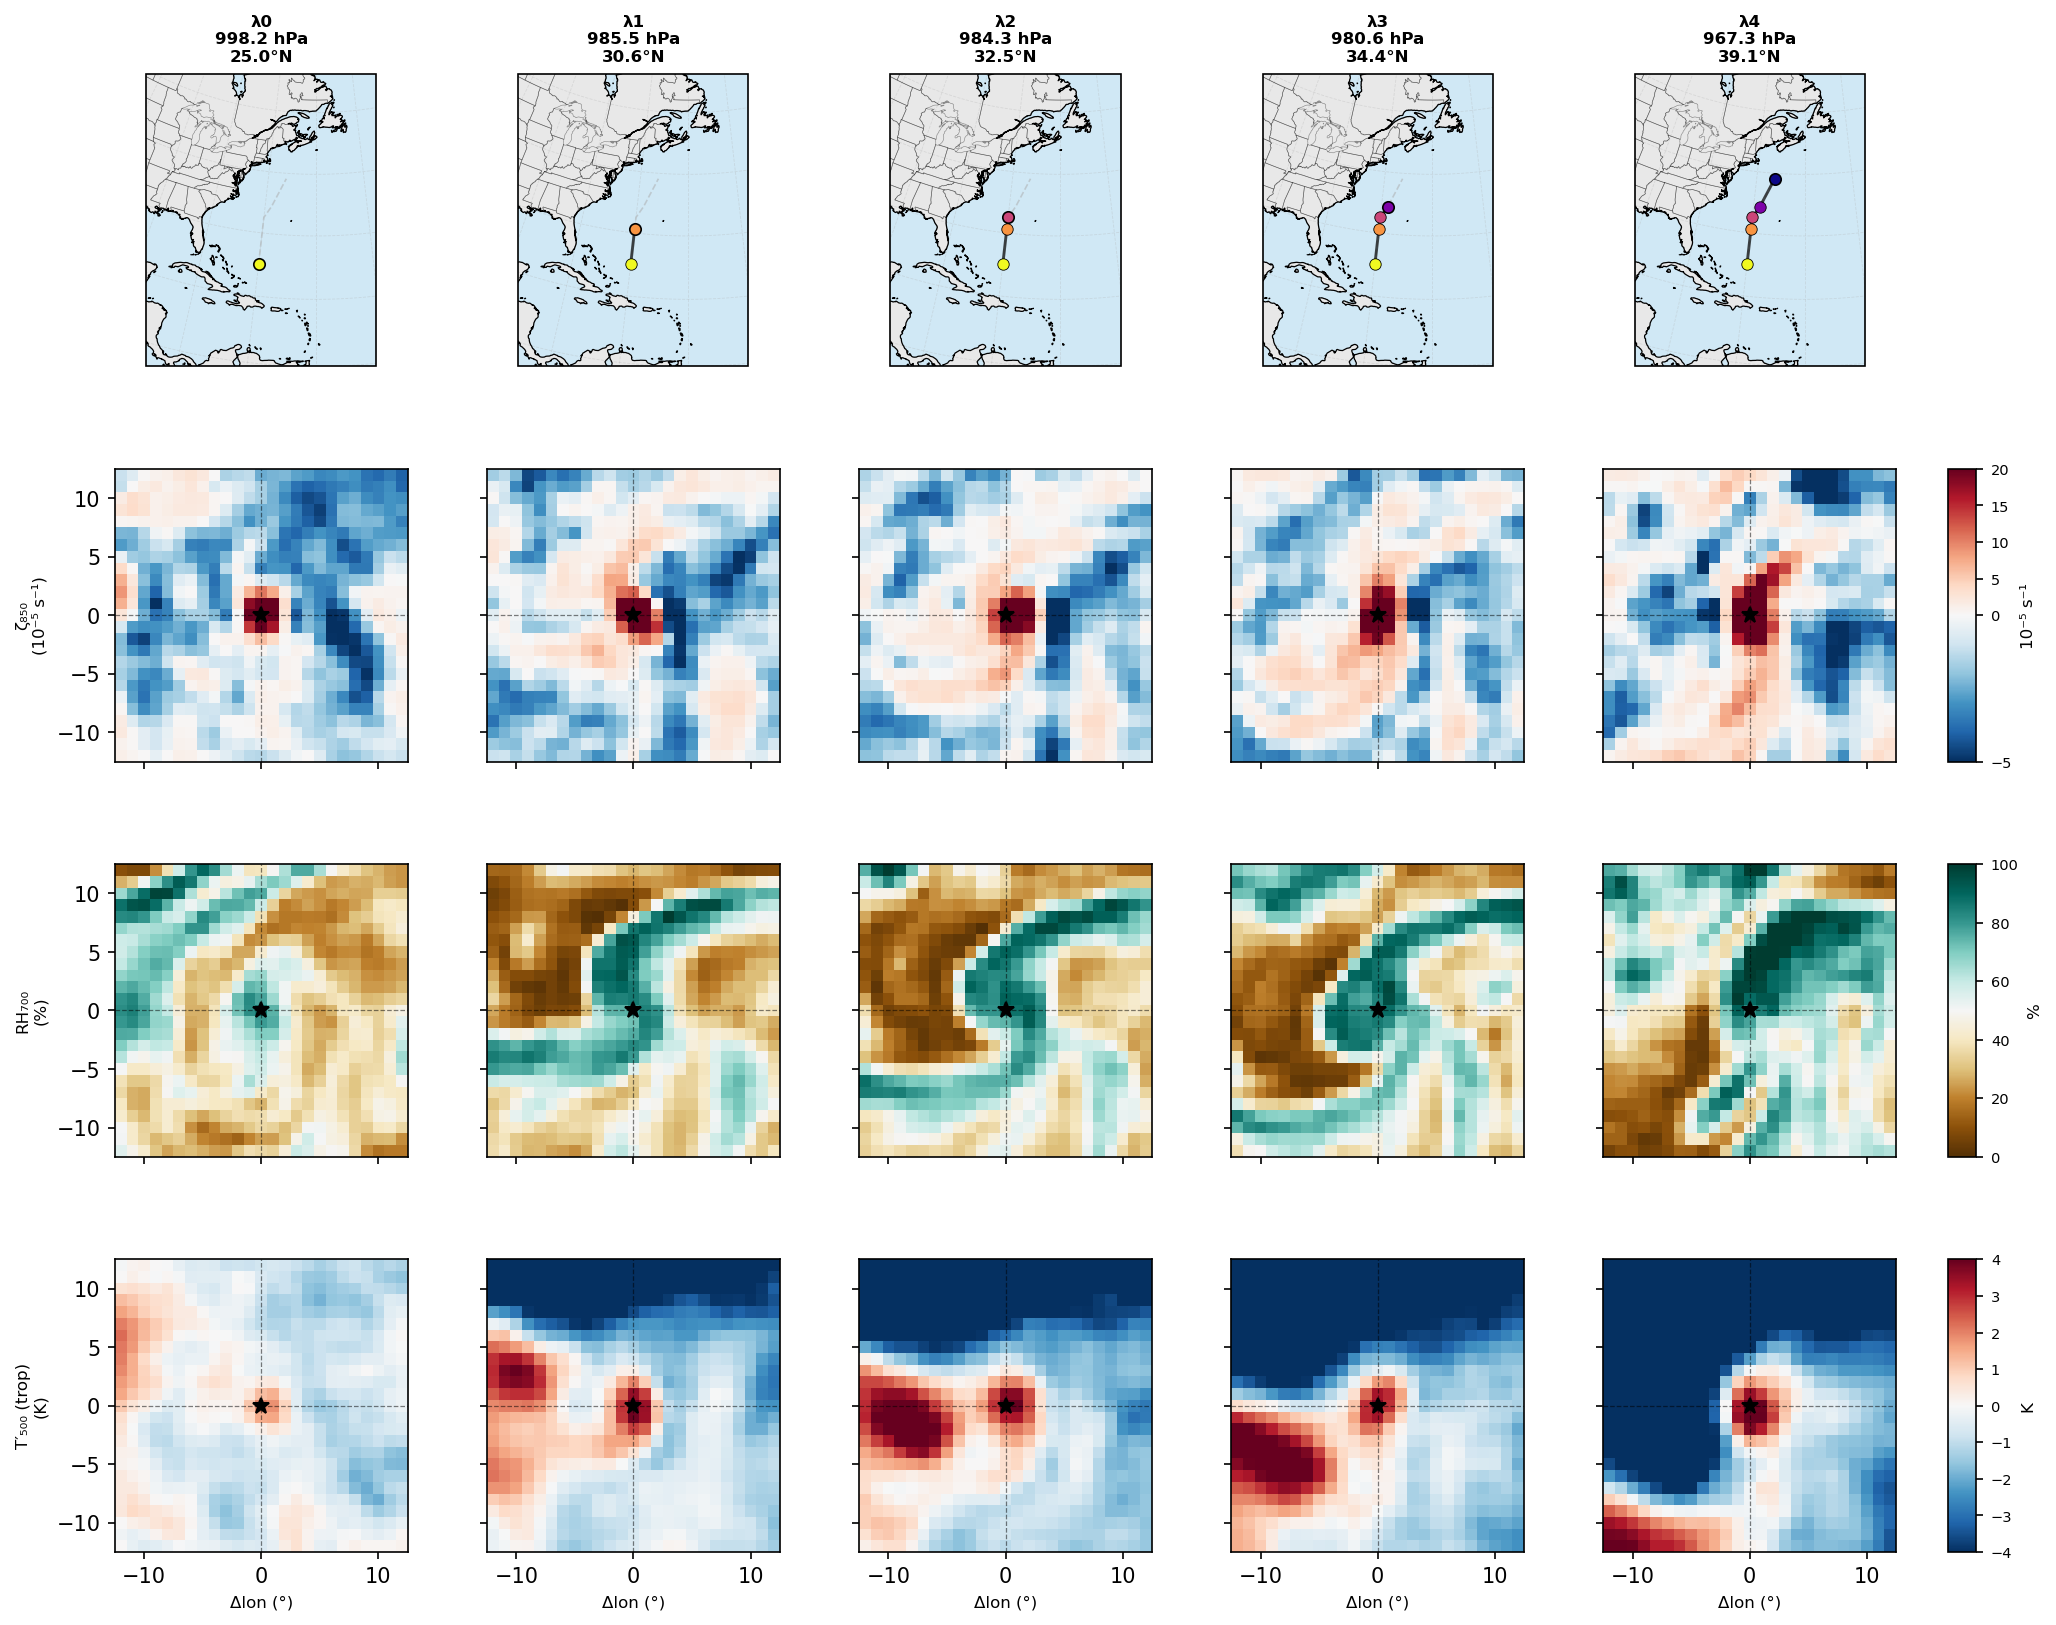
\includegraphics[width=\textwidth]{trajectory_2022-09-02T00Z_pathway26.png}
\caption{Storm-centred physics along a representative reactive pathway for the Earl IC
(2022-09-02T00Z, pathway~26), $\lambda_0$ through $\lambda_4$.
Each column shows one interface crossing; column headers give the MSLP and storm latitude.
The vortex tracks northeastward from 25$^\circ$N at $\lambda_0$ to 39$^\circ$N at $\lambda_4$,
consistent with typical late-summer Atlantic tracks in this environment.
\textit{Row 1}: 850-hPa relative vorticity $\zeta_{850}$ ($10^{-5}$~s$^{-1}$).
\textit{Row 2}: 700-hPa relative humidity RH$_{700}$ (\%).
\textit{Row 3}: 500-hPa warm-core anomaly $T'_{500}$ (K, relative to 0--30$^\circ$N mean).
The persistent cyclonic vorticity and warm-core anomaly at each interface confirm continuous
vortex identity and warm-core structure through state~$B$.
Pathways where the warm core collapses at high latitudes are screened out by the CPS filter
and not included in the genesis rate calculation.}
\label{fig:physics}
\end{figure}

\subsection{Storm-Centred Physics Composites}

Figures~\ref{fig:composites_earl}--\ref{fig:composites_ian} show storm-centred composites
of vorticity, relative humidity, and warm-core anomaly, composited across all reactive
pathways for each case-study IC.
By averaging over all configurations that successfully reach state~$B$, these composites
reveal the mean thermodynamic and kinematic environment that supports genesis, smoothing
out pathway-to-pathway variability to expose the underlying physical signal.

All three ICs share a common structural signature: a compact positive vorticity core at
850~hPa, a saturated inner core (RH$_{700} \gtrsim 70\%$), and a growing warm-core anomaly
at 500~hPa that strengthens progressively from $\lambda_0$ through state~$B$.
The amplitude of $T'_{500}$ at state~$B$ is comparable across the three cases despite their
differing genesis rates, suggesting that once a vortex reaches state~$B$ it has traversed
a physically similar intensification pathway regardless of the environmental background.
The primary inter-IC difference appears at early interfaces: the Earl IC composites
show weaker vorticity and warm-core organisation at $\lambda_1$--$\lambda_2$ compared
to the Fiona and Ian composites, directly reflecting the lower $P_1$ value for Earl
(Table~\ref{tab:results}) and confirming that the conditional probability bottleneck
has a physically interpretable composite signature.

\begin{figure}[htbp]
\centering
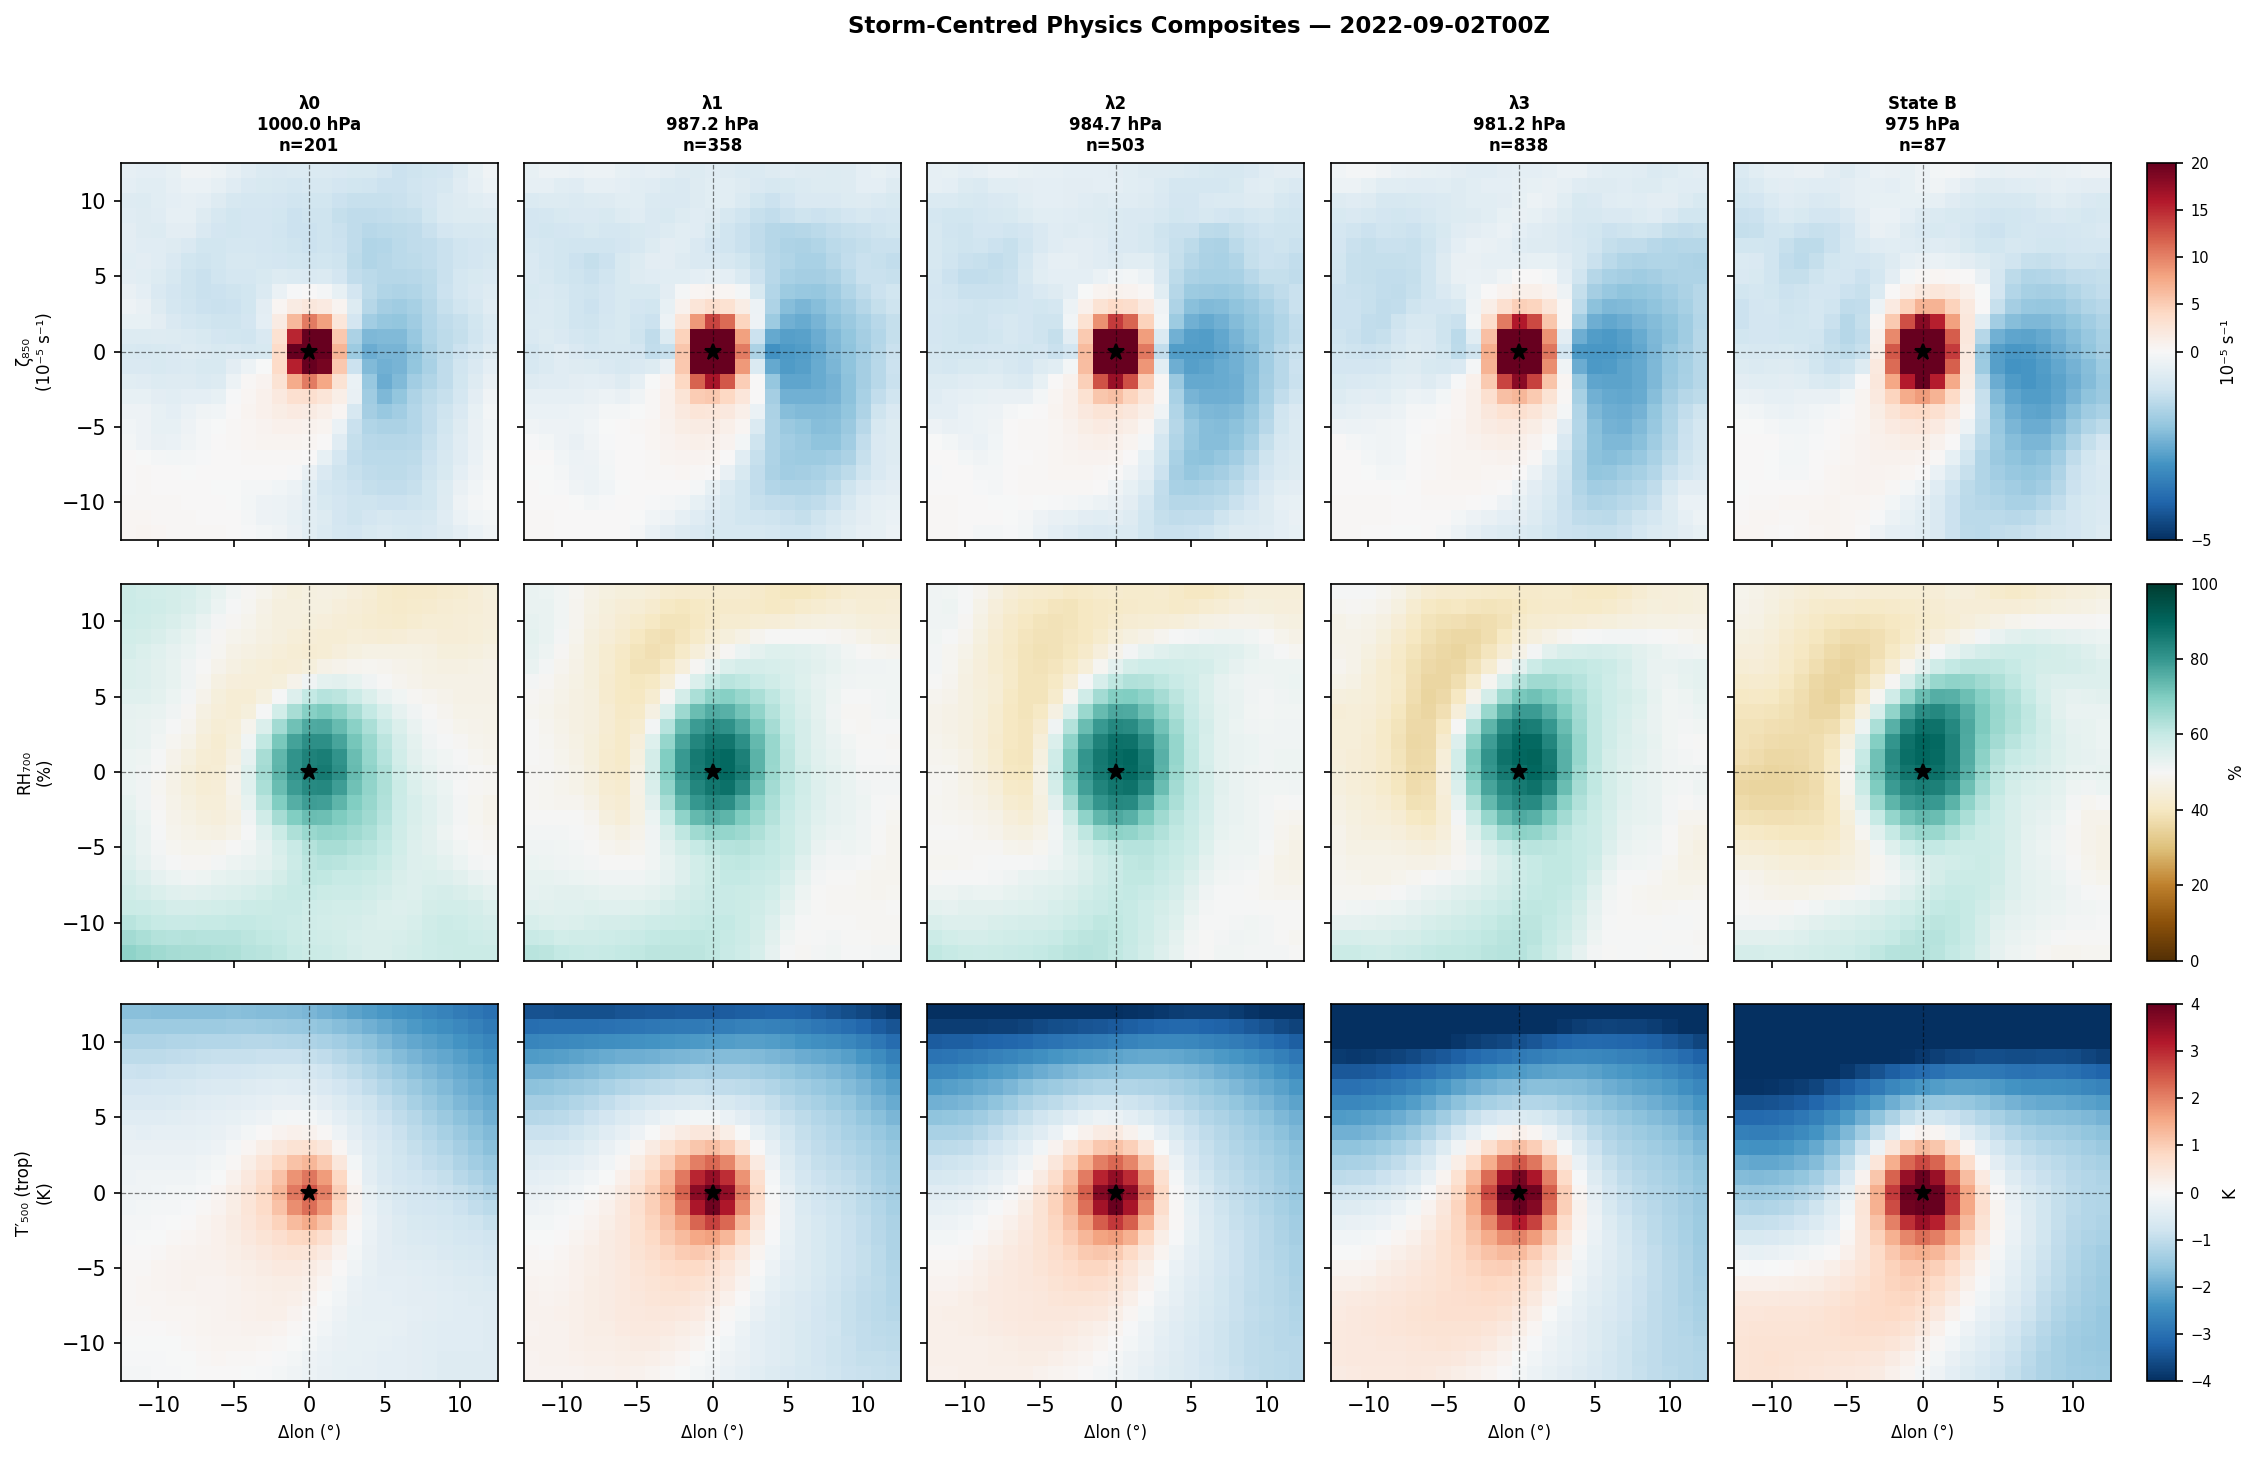
\includegraphics[width=\textwidth]{2022-09-02T00Z_composites.png}
\caption{Storm-centred physics composites along reactive pathways for the Earl IC
(2022-09-02T00Z). Columns show interfaces $\lambda_0$ through state~$B$; sample sizes
$n$ in each column header. Rows show: (1) 850-hPa relative vorticity $\zeta_{850}$
($10^{-5}$~s$^{-1}$); (2) 700-hPa relative humidity RH$_{700}$ (\%);
(3) 500-hPa warm-core anomaly $T'_{500}$ (K).
The weaker vorticity and warm-core organisation at $\lambda_1$ reflects Earl's
lower $P_1$ value and identifies initial organisation as the rate-limiting bottleneck.}
\label{fig:composites_earl}
\end{figure}

\begin{figure}[htbp]
\centering
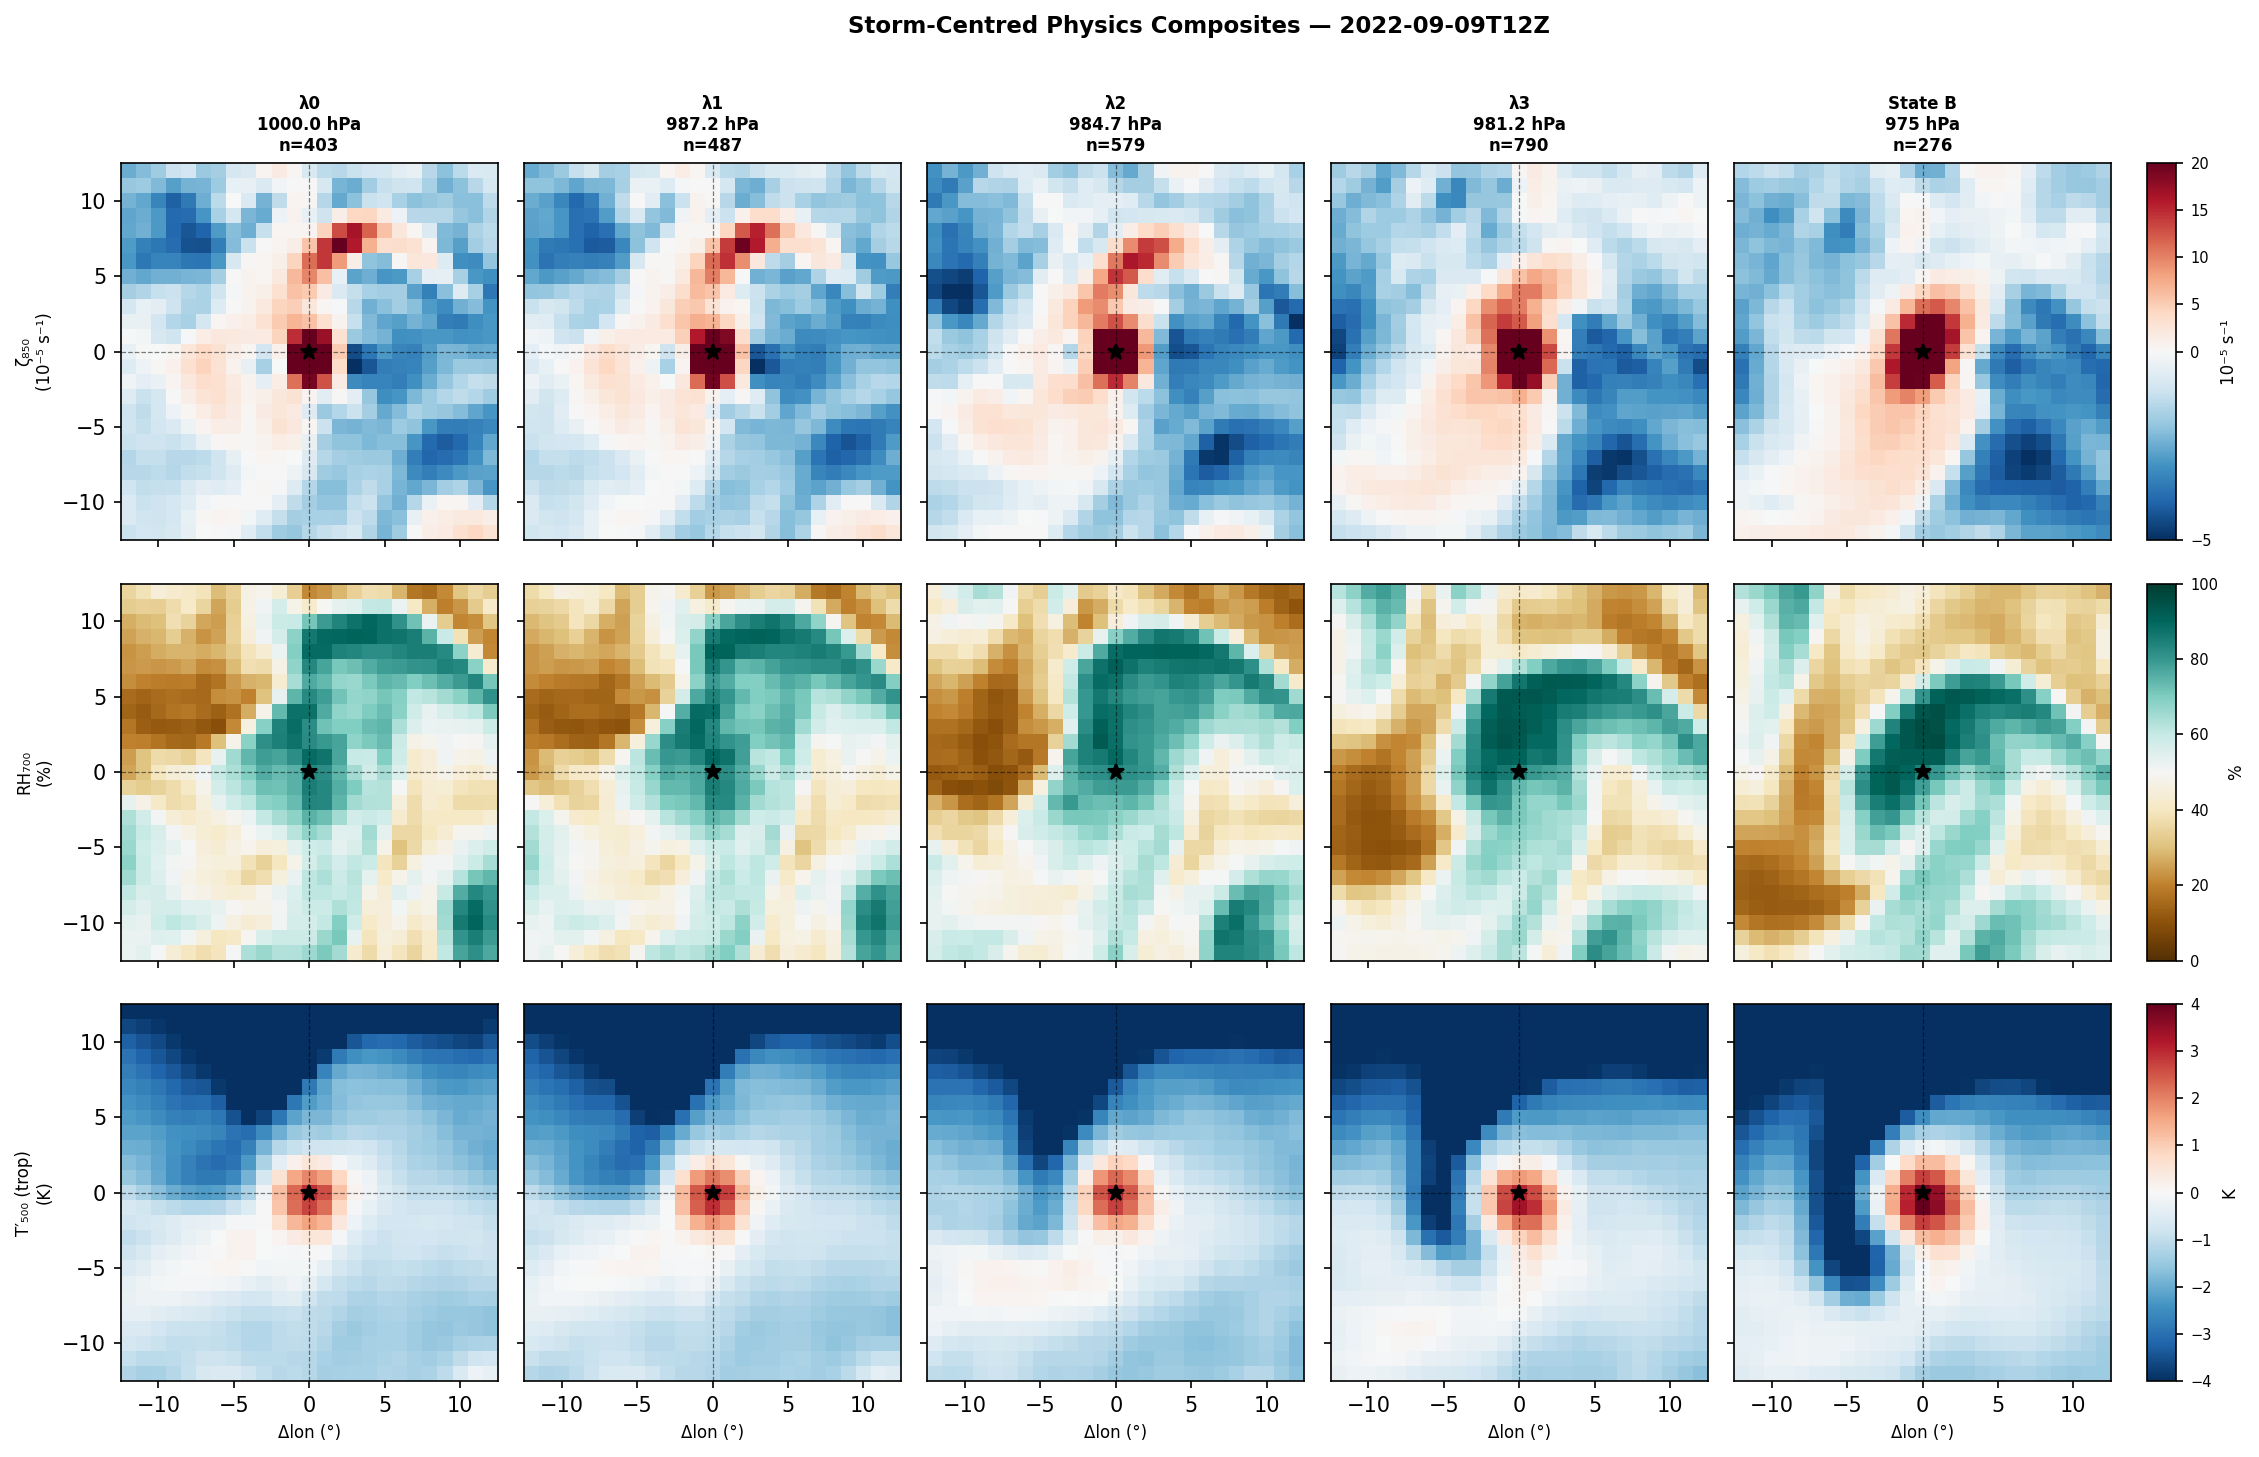
\includegraphics[width=\textwidth]{2022-09-09T12Z_composites.png}
\caption{As in Fig.~\ref{fig:composites_earl} but for the Fiona precursor IC
(2022-09-09T12Z). Stronger vorticity and warm-core development at early interfaces
compared to Earl reflects the more favourable large-scale environment and higher $P_1$.}
\label{fig:composites_fiona}
\end{figure}

\begin{figure}[htbp]
\centering
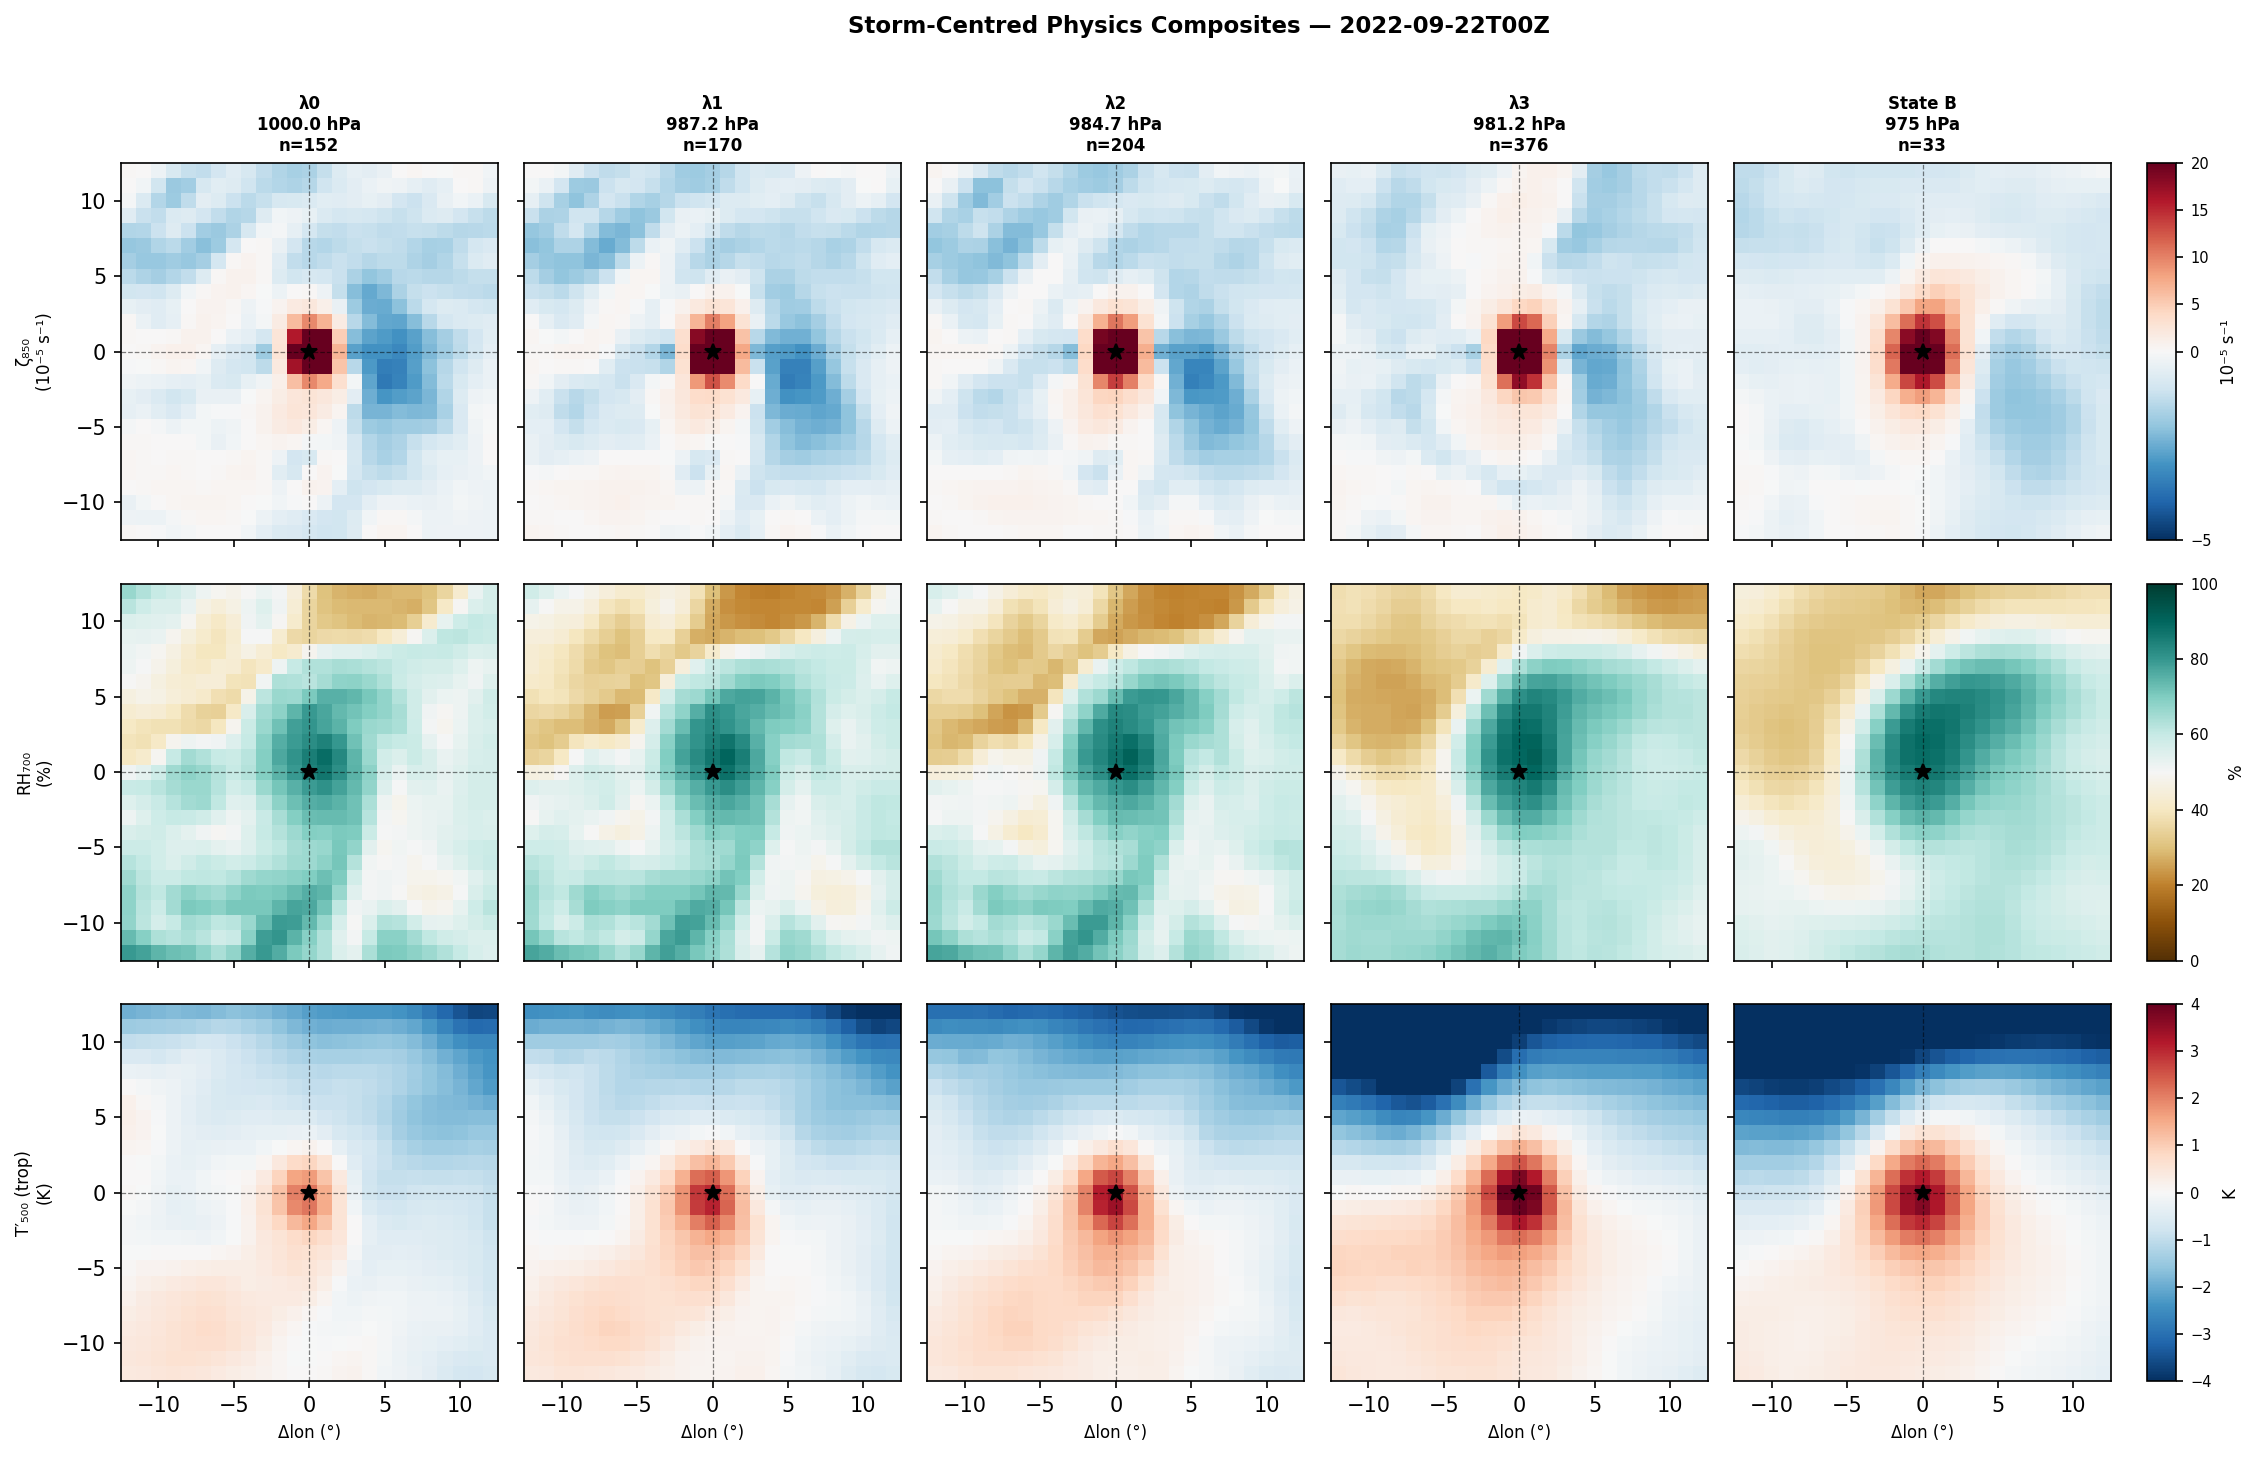
\includegraphics[width=\textwidth]{2022-09-22T00Z_composites.png}
\caption{As in Fig.~\ref{fig:composites_earl} but for the Ian precursor IC
(2022-09-22T00Z). The $T'_{500}$ amplitude at state~$B$ is comparable across all three
ICs despite their differing genesis rates, suggesting a physically similar final
intensification pathway once the vortex reaches the near-hurricane threshold.}
\label{fig:composites_ian}
\end{figure}

\section{Discussion and Conclusions}

\subsection{Methodological Validation and Practical Considerations}

The central validation result --- FFS and direct-sampling rates agreeing within
$1.03\pm0.15$ across 98 initial conditions --- provides strong empirical support for
the method. These are entirely independent estimates derived from the same simulation
data: the FFS rate uses only the interface crossing counts and shooting probabilities,
while the direct rate uses only the raw state-$B$ arrival counts from flux trajectories.
Their close agreement across three orders of magnitude of genesis probability confirms
that (1) the interface spacing produces well-conditioned conditional probability estimates,
(2) the ensemble sizes ($N=2000$ per interface) are sufficient, and (3) the CPS
contamination screen does not introduce systematic bias.

Enhancement factors (3--140$\times$, geometric mean 14$\times$)
scale inversely with genesis probability, as expected from FFS theory \citep{allen2009forward}.
The right-skewed speedup distribution mirrors the log-normal FFS rate distribution itself;
the geometric mean is the appropriate summary for such distributions and is reported throughout.
For the most active environments where direct sampling is feasible (speedup $3\times$), the two
methods serve as mutual validation. For suppressed environments (speedup $\sim$100$\times$),
FFS is the only practical route to a quantitative genesis rate estimate.

The bottleneck analysis adds physical content beyond a scalar rate. For the Earl IC,
the rate-limiting step at $\lambda_1$ (initial organization) indicates that the
environment is resistant to producing organized convection but that once organized,
the system is likely to reach hurricane strength. For the Ian precursor IC, the
easy initial organization but hard final intensification ($P_4 = 0.102$) suggests
an environment whose large-scale structure is favorable for genesis attempts but
where the thermodynamic pathway to full hurricane development requires specific
mesoscale alignment not yet present 24~hours before NHC designation.

The CPS filter warrants clarification. At 1$^\circ$ resolution, formal CPS parameters
are not quantitatively validated against higher-resolution analyses, and our implementation
omits the thermal asymmetry ($B$) parameter. The filter is best understood as a
contamination screen rather than a rigorous warm-core classifier --- rejecting obviously
extratropical systems while accepting all ambiguous cases. Future implementations with
finer-resolution models could apply a more principled multidimensional CPS criterion.

\subsection{Limitations}

This study analyzes a single hurricane season (2022). Interannual variability driven
by ENSO, the AMO, and Saharan dust outbreaks is not represented. The SDL-WXFormer was
trained on ERA5 (1979--2021) at 1$^\circ$ resolution, which smooths intense vortex
cores and underrepresents Category~3+ hurricanes; state~$B$ is accordingly defined at
975~hPa rather than the intensities typical of major hurricane activity. Validation
against physics-based models (WRF, IFS) at higher resolution is an important next step.

Additionally, MSLP as an order parameter has known limitations at 1$^\circ$ resolution:
terrain-induced pressure artifacts (present in this model due to topographic interpolation
differences) require the CPS filter and geographic masking described in Section~2.3.
More fundamentally, MSLP does not capture the thermodynamic and kinematic prerequisites
for genesis --- warm-core development, vorticity alignment, mid-level moistening, shear
suppression --- that precede a detectable surface pressure signature.
A disturbance can cross $\lambda_0 = 1000$~hPa as a transient trough with no tropical
development potential, and the FFS rate therefore measures the frequency of organised
\textit{MSLP} deepening rather than tropical genesis in a dynamically complete sense.
Reaction coordinates based on vorticity, saturation fraction, or a composite genesis
potential index \citep[e.g.,][]{bister1998dissipative,camargo2007use}
would provide a more physically targeted order parameter; such extensions are deferred
to future work but are expected to improve both the enhancement factor and the
physical interpretability of the per-interface bottleneck diagnostics.

\subsection{Conclusions}

Forward Flux Sampling resolves Atlantic tropical cyclogenesis rates spanning three orders
of magnitude from 98 atmospheric initial conditions in a fast neural weather emulator,
with internal validation confirming FFS and direct-sampling rates agree within 3\%.
Computational enhancement of 3--140$\times$ (geometric mean $14\times$) makes FFS
practical across the full range of synoptic environments. Physically, the method reveals
that the rate-limiting step in genesis varies by regime: initial tropical organization
($P_1$ bottleneck, as in Earl), uniformly elevated crossing probabilities with a terminal
intensification barrier ($P_4$ bottleneck, as in the active-period IC), or a compound
barrier at the final intensification stages ($P_3$--$P_4$, as in the Ian precursor).
These distinct bottleneck signatures encode mechanistic information about genesis pathway
dynamics that is invisible to scalar rate estimates from direct sampling.

The methodology extends directly to other atmospheric rare events (extreme heatwaves,
sudden stratospheric warmings, blocking onset) and to physics-based models. The
combination of neural emulators with rare event sampling opens a computationally
tractable path to systematic characterization of low-probability, high-consequence
atmospheric events across climatic regimes.

\appendix
\section{Supplementary Information: State-$B$ Threshold Sensitivity}
\label{sec:si_threshold}

The choice of $\lambda_B = 975$~hPa was arrived at empirically.
Initial experiments used $\lambda_B = 965$~hPa, targeting stronger tropical storm
to Category~1 intensity. Two systematic problems emerged at this threshold:
(1) state-$B$ arrivals were disproportionately located at latitudes $>40^\circ$N,
where the SDL-WXFormer's 1$^\circ$ MSLP field deepens in association with
extratropical systems that the simplified CPS filter could not reliably reject
at this intensity; (2) the conditional probability $P_4$ collapsed toward values
$<0.05$ across most ICs, concentrating nearly all the variance in the final interface
and producing highly skewed speedup distributions that degraded FFS efficiency.

Raising $\lambda_B$ to 975~hPa resolved both issues: state-$B$ arrivals shifted to
the tropical and subtropical Atlantic/Caribbean/Gulf domain consistent with observed
genesis climatology (Figure~\ref{fig:stateb_geo}), and the four $P_i$ values
distributed more uniformly, maintaining the well-conditioned range (0.25--0.75)
targeted by the interface placement algorithm.

The sensitivity of reported genesis \textit{rates} to threshold choice is expected:
$k(\lambda_B = 975)$ and $k(\lambda_B = 965)$ differ by roughly one order of magnitude,
consistent with the additional conditional probability factor for the extra interface.
The key methodological properties --- internal self-consistency, seasonal cycle
structure, and bottleneck diagnostics --- are qualitatively robust across thresholds.
For physics-based models at finer resolution, a lower $\lambda_B$ (e.g., 960~hPa)
may be more appropriate, and the interface placement should be re-optimised accordingly.

\section*{Acknowledgments}
The author thanks colleagues at NCAR's Earth System Data Science group for discussions
on neural weather prediction. Computational resources provided by the
NCAR-Wyoming Supercomputing Center (Derecho and Casper systems) supported this research.
This work was supported by NSF grants AGS-XXXXXX and CSSI-XXXXXX.

\section*{Data Availability Statement}
The FFS driver code, vortex tracker, and contamination screen are available at
\url{https://github.com/NCAR/miles-tails}.
Note that \texttt{config/ffs.yml} in the repository reflects a development-phase
parameter set; the operative interface values and thresholds are those stated in
Section~2.1 of this paper.
The FFS simulation output (rate statistics, conditional crossing probabilities, and
reactive pathway summaries for all 98 initial conditions) will be archived at the
NCAR Research Data Archive upon acceptance.
ERA5 reanalysis initial conditions are available from the Copernicus Climate Data Store
(\url{https://cds.climate.copernicus.eu}).
IFS ensemble data are available through WeatherBench2 \citep{rasp2024weatherbench2}.
\textbf{[SDL-WXFormer model weights: update repository link before submission.]}

% ametsoc.bst not in local TeX Live — download from https://www.ametsoc.org/ams/index.cfm/publications/authors/journal-and-bams-authors/author-resources/latex-author-info/
% For JAMES submission swap plainnat -> ametsoc (or agu if using AGU template).
\bibliographystyle{plainnat}
\bibliography{references}

\end{document}
